\chapter{Экспериментальное исследование и сравнительный анализ эффективности предложенной системы}
\label{ch:4}

	\section{Эксперимент дообучения рассматриваемых нейронных сетей}
\label{sec:experement}

Для адаптации ранее обученной нейронной сети в реальных условиях оператор
располагает возможностью провести 1--2 калибровочных полёта в целевом районе
перед основной миссией.
Целью данного эксперимента является построение зависимости между долей
дообучающего датасета и точностью восстановленной траектории~RMSE.
По результатам эксперимента предлагается сводная рекомендательная таблица
с зависимостью между длинами потери сигнала ГНСС и долями дообучающей выборки
для предлагаемой нейронной сети.

% =========================================================
\subsection{Характеристика экспериментальных данных}
\label{sec:datasets}
% =========================================================

Эксперименты проводились на двух датасетах, полученных в симуляторе
PX4/Gazebo~\cite{Burri2016}:
\begin{itemize}
	\item \textbf{Датасет~A (стандартный режим):} полёты в спокойных условиях
	с ограниченными манёврами; номинальный сценарий горизонтального облёта
	промышленного объекта. Все четыре модели предобучались на данном датасете.
	\item \textbf{Датасет~B (режим компенсации порывов ветра):} полёты с резкими
	изменениями скорости и направления, имитирующими компенсацию порывов ветра
	вблизи промышленной конструкции. В данном сценарии дисперсия оборотов
	двигателей максимальна. Общая продолжительность составила 8~мин 42~с.
\end{itemize}

Оба датасета содержат синхронизированные данные БИНС (200~Гц), ГНСС (5~Гц),
телеметрию оборотов двигателей (200~Гц) и опорные траектории от внутреннего
состояния симулятора.
Предобучение выполнялось на датасете~A, дообучение --- на подмножествах
датасета~B.
Ключевые статистики датасетов приведены в таблице~\ref{tab:dataset}.

\begin{table}[htbp]
	\centering
	\caption{Сравнение статистических характеристик датасетов A и B\\
		\textit{Table~2. Statistical characteristics of datasets A and B}}
	\label{tab:dataset}
	\begin{tabular}{l *{3}{c}}
		\toprule
		{Показатель} &
		\multicolumn{1}{c}{Датасет~A} &
		\multicolumn{1}{c}{Датасет~B} &
		\multicolumn{1}{c}{Отношение B/A} \\
		\midrule
		\multicolumn{4}{l}{\textit{Линейная скорость $|\mathbf{v}|$, м/с}} \\
		\quad среднее & \num{1.790} & \num{2.332} & \num{1.30} \\
		\quad std & \num{0.767} & \num{2.097} & \num{2.74} \\
		\quad p95 & \num{3.253} & \num{6.743} & \num{2.07} \\
		\midrule
		\multicolumn{4}{l}{\textit{Горизонтальное ускорение $|a_{xy}|$, м/с²}} \\
		\quad среднее & \num{0.131} & \num{0.293} & \num{2.24} \\
		\quad std & \num{0.088} & \num{0.263} & \num{3.00} \\
		\quad p95 & \num{0.313} & \num{0.832} & \num{2.66} \\
		\midrule
		\multicolumn{4}{l}{\textit{Угловая скорость $|\boldsymbol{\omega}|$, рад/с}} \\
		\quad среднее & \num{0.321} & \num{0.292} & \num{0.91} \\
		\quad p95 & \num{0.913} & \num{0.942} & \num{1.03} \\
		\midrule
		\multicolumn{4}{l}{\textit{Средние обороты роторов, об/мин}} \\
		\quad среднее & \num{14545} & \num{11566} & \num{0.80} \\
		\quad \textbf{std} & \textbf{\num{990}} & \textbf{\num{5971}} & \textbf{\num{6.03}} \\
		\quad p95 & \num{16150} & \num{15265} & \num{0.95} \\
		\bottomrule
	\end{tabular}
\end{table}

Данные таблицы~\ref{tab:dataset} позволяют сформулировать три ключевых вывода.
Во-первых, средняя скорость в датасете~B на 30\% выше, а горизонтальное
ускорение в~2{,}2~раза; угловые скорости практически идентичны
(отношение 0{,}91--1{,}03), что означает: режим компенсации порывов ветра
не сводится к простому ускорению платформы.
Во-вторых, стандартное отклонение оборотов в датасете~B в \textbf{6{,}0~раза}
превышает таковое в датасете~A (5971 против 990~об/мин), тогда как среднее
значение оборотов ниже (11566 против 14545~об/мин): при компенсации ветровых
возмущений квадрокоптер совершает частые асимметричные изменения тяги
отдельных роторов, сохраняя суммарную тягу вблизи~$F_z \approx mg$.
В-третьих, БИНС измеряет суммарное специфическое ускорение и не различает
дифференциальные изменения тяги роторов, тогда как телеметрия оборотов
непосредственно фиксирует эти изменения.
Таким образом, сигналы БИНС и оборотов несут взаимодополняющую информацию:
БИНС обеспечивает достаточную точность при умеренных манёврах, сигнал оборотов
повышает контраст обучающего сигнала при дообучении именно там, где БИНС
теряет информативность.

% =========================================================
\subsection{Результаты дообучения при ограниченных данных}
\label{sec:exp2}
% =========================================================

Из датасета~B случайно отбирались подмножества долей 10, 25, 50, 75 и 100\%.
Число шагов оптимизации фиксировалось на уровне 2000 для всех долей,
что исключает влияние числа итераций на результат и обеспечивает
сопоставимость условий дообучения.
Оценка проводилась на 10 случайных сегментах датасета~B методом
среднеквадратического отклонения без совмещения систем координат.
Набор результатов охватывает 4~модели $\times$ 5~долей $\times$ 6~длительностей
потери сигнала (3, 10, 30, 60, 120 и 240~с), что соответствует 120 численным
значениям RMSE.

На основе полученных данных выявлен лучший и наиболее сложный сценарии для
предлагаемой нейронной сети.
В таблице~\ref{tab:rmse_60} представлены результаты при потере сигнала 60~с
(лучший сценарий).
При такой длительности накопленная ошибка БИНС ещё не достигает критических
значений, и все четыре модели демонстрируют сравнительно малые RMSE.
Тем не менее предлагаемая нейронная сеть стабильно превосходит базовую при
всех долях датасета~B.

\begin{table}[htbp]
	\centering
	\caption{RMSE (м) при дообучении на подмножествах, потеря сигнала ГНСС 60~с
		\emph{(лучший сценарий)}\\
		\textit{Table~3. RMSE (m) for fine-tuning on subsets, GNSS outage 60~s (best-case scenario)}}
	\label{tab:rmse_60}
	\begin{tabular}{c >{\columncolor{blue!8}}c *{3}{c}}
		\toprule
		Доля, \% &
		\makecell[tc]{\textbf{предлагаемая} \\ \textbf{нейронная} \\ \textbf{сеть}} &
		\makecell[tc]{\textbf{обобщённая} \\ \textbf{нейронная} \\ \textbf{сеть}} &
		\makecell[tc]{\textbf{базовая} \\ \textbf{нейронная} \\ \textbf{сеть}} &
		\textbf{Transformer} \\
		\midrule
		10  & \textbf{\num{1,973}} & \num{2,163} & \num{2,985} & \num{5,800} \\
		25  & \num{2,232} & \textbf{\num{2,031}} & \num{3,085} & \num{6,797} \\
		50  & \textbf{\num{2,017}} & \num{1,739} & \num{3,477} & \num{7,488} \\
		75  & \textbf{\num{3,029}} & \num{2,457} & \num{3,454} & \num{8,737} \\
		100 & \textbf{\num{3,647}} & \num{3,777} & \num{6,994} & \num{5,657} \\
		\bottomrule
	\end{tabular}
\end{table}

В таблице~\ref{tab:rmse_240} представлены результаты при потере сигнала 240~с
(наиболее сложный сценарий).
При такой длительности ошибка БИНС нарастает до десятков метров, и различия
в регуляризующих свойствах моделей проявляются в наибольшей степени.
Transformer демонстрирует стабильно высокую ошибку при всех долях данных,
что объясняется квадратичной сложностью механизма внимания при обработке
длинных последовательностей навигационных данных.

\begin{table}[htbp]
	\centering
	\caption{RMSE (м) при дообучении на подмножествах, потеря сигнала ГНСС 240~с
		\emph{(наиболее сложный сценарий)}\\
		\textit{Table~4. RMSE (m) for fine-tuning on subsets, GNSS outage 240~s (worst-case scenario)}}
	\label{tab:rmse_240}
	\begin{tabular}{c >{\columncolor{blue!8}}c *{3}{c}}
		\toprule
		{Доля, \%} &
		\makecell[tc]{\textbf{предлагаемая} \\ \textbf{нейронная} \\ \textbf{сеть}} &
		\makecell[tc]{\textbf{обобщённая} \\ \textbf{нейронная} \\ \textbf{сеть}} &
		\makecell[tc]{\textbf{базовая} \\ \textbf{нейронная} \\ \textbf{сеть}} &
		\textbf{Transformer} \\
		\midrule
		10  & \textbf{\num{14,273}} & \num{19,985} & \num{36,458} & \num{22,315} \\
		25  &         \num{9,409}  & \textbf{\num{8,173}}  & \num{13,016} & \num{20,267} \\
		50  & \textbf{\num{10,594}} & \num{13,412} & \num{21,823} & \num{19,593} \\
		75  & \textbf{\num{15,069}} & \num{20,264} & \num{32,100} & \num{20,963} \\
		100 &  \textbf{\num{9,734}} & \num{11,149} & \num{16,978} & \num{20,481} \\
		\bottomrule
	\end{tabular}
\end{table}

\subsection{Сводная таблица по всем режимам}

Таблица~\ref{tab:summary_df} представляет полный обзор результатов предлагаемой
нейронной сети по всем 6 длинам потери сигнала и всем 5 долям дообучающего
датасета.
Данная таблица может служить операционным руководством для оценки требуемого
объёма калибровочного полёта в новых динамических условиях.

\begin{table}[htbp]
	\centering
	\caption{RMSE (м) предлагаемой нейронной сети по всем длинам потери сигнала и долям датасета (сводная таблица)\\
		\textit{Table~5. RMSE (m) of the proposed neural network for all outage durations and dataset fractions (summary)}}
	\label{tab:summary_df}
	\begin{tabular}{c *{6}{c}}
		\toprule
		\multirow{2}{*}{Доля датасета, \%} &
		\multicolumn{6}{c}{Длина потери сигнала ГНСС, с} \\
		\cmidrule(lr){2-7}
		& {3} & {10} & {30} & {60} & {120} & {240} \\
		\midrule
		10  & \num{0,141} & \num{0,511} & \num{1,722} & \num{1,973} & \num{6,723}  & \num{14,273} \\
		25  & \num{0,133} & \num{0,785} & \num{2,463} & \num{2,232} & \num{7,264}  & \num{9,409}  \\
		50  & \num{0,124} & \num{0,731} & \num{1,764} & \num{2,017} & \num{6,689}  & \num{10,594} \\
		75  & \num{0,095} & \num{0,690} & \num{2,150} & \num{3,029} & \num{5,505}  & \num{15,069} \\
		100 & \num{0,104} & \num{0,571} & \num{1,936} & \num{3,647} & \num{9,458}  & \num{9,734}  \\
		\bottomrule
	\end{tabular}
\end{table}

При коротких потерях сигнала (3--30~с) предлагаемая нейронная сеть обеспечивает
RMSE ниже 2{,}5~м при любой доле обучающих данных.
При длительных потерях (120--240~с) оптимальная доля данных составляет 25--50\%,
что соответствует 2--4~мин калибровочных полётов перед миссией.

\subsection{Визуализация результатов}

Рисунок~\ref{fig:rmse_plot} иллюстрирует RMSE всех четырёх моделей при
потере сигнала 240~с в зависимости от доли обучающих данных.
Предлагаемая нейронная сеть и обобщённая нейронная сеть устойчиво превосходят
базовую при всех долях; Transformer сохраняет стабильно высокую ошибку и
практически не улучшается с увеличением объёма данных дообучения.

\begin{figure}[htbp]
	\centering
	\resizebox{0.92\linewidth}{!}{% plot.tex — RMSE четырёх моделей при потере сигнала 240 с
% Подключать как: \resizebox{0.92\linewidth}{!}{% plot.tex — RMSE четырёх моделей при потере сигнала 240 с
% Подключать как: \resizebox{0.92\linewidth}{!}{% plot.tex — RMSE четырёх моделей при потере сигнала 240 с
% Подключать как: \resizebox{0.92\linewidth}{!}{\input{../src/plot.tex}}
% Требует в преамбуле: \usepackage{pgfplots}, \usetikzlibrary{patterns}

\begin{tikzpicture}
\begin{axis}[
  ybar,
  bar width      = 7pt,
  width          = \linewidth,
  height         = 7.5cm,
  legend style   = {at={(0.5,-0.28)}, anchor=north, legend columns=2,
                    font=\small, draw=black},
  xlabel         = {Доля обучающих данных, \%},
  ylabel         = {СКО, м},
  xlabel style   = {font=\small},
  ylabel style   = {font=\small},
  xtick          = {1,2,3,4,5},
  xticklabels    = {10, 25, 50, 75, 100},
  xticklabel style = {font=\small},
  yticklabel style = {font=\small},
  ymin           = 0,
  ymax           = 42,
  ymajorgrids    = true,
  grid style     = {dashed, gray!40},
  enlarge x limits = 0.12,
  nodes near coords,
  nodes near coords style = {font=\tiny, rotate=90, anchor=west,
                             xshift=2pt, yshift=0pt},
  every node near coord/.append style={/pgf/number format/fixed,
                                        /pgf/number format/precision=1},
]

% НС ПСПС-ДФ (синий)
\addplot[
  fill=blue!60,
  draw=blue!80!black,
  line width=0.8pt
] coordinates {
  (1, 14.273)
  (2,  9.409)
  (3, 10.594)
  (4, 15.069)
  (5,  9.734)
};

% НС ПСПС-КФ (зелёный)
\addplot[
  fill=green!55!black,
  draw=green!70!black,
  line width=0.8pt
] coordinates {
  (1, 19.985)
  (2,  8.173)
  (3, 13.412)
  (4, 20.264)
  (5, 11.149)
};

% НС ПСПС-Б (красный)
\addplot[
  fill=red!65,
  draw=red!80!black,
  line width=0.8pt
] coordinates {
  (1, 36.458)
  (2, 13.016)
  (3, 21.823)
  (4, 32.100)
  (5, 16.978)
};

% Transformer (оранжевый)
\addplot[
  fill=orange!70,
  draw=orange!90!black,
  line width=0.8pt
] coordinates {
  (1, 22.315)
  (2, 20.267)
  (3, 19.593)
  (4, 20.963)
  (5, 20.481)
};

\legend{предлагаемая, обобщенная, базовая, Transformer}
\end{axis}
\end{tikzpicture}
}
% Требует в преамбуле: \usepackage{pgfplots}, \usetikzlibrary{patterns}

\begin{tikzpicture}
\begin{axis}[
  ybar,
  bar width      = 7pt,
  width          = \linewidth,
  height         = 7.5cm,
  legend style   = {at={(0.5,-0.28)}, anchor=north, legend columns=2,
                    font=\small, draw=black},
  xlabel         = {Доля обучающих данных, \%},
  ylabel         = {СКО, м},
  xlabel style   = {font=\small},
  ylabel style   = {font=\small},
  xtick          = {1,2,3,4,5},
  xticklabels    = {10, 25, 50, 75, 100},
  xticklabel style = {font=\small},
  yticklabel style = {font=\small},
  ymin           = 0,
  ymax           = 42,
  ymajorgrids    = true,
  grid style     = {dashed, gray!40},
  enlarge x limits = 0.12,
  nodes near coords,
  nodes near coords style = {font=\tiny, rotate=90, anchor=west,
                             xshift=2pt, yshift=0pt},
  every node near coord/.append style={/pgf/number format/fixed,
                                        /pgf/number format/precision=1},
]

% НС ПСПС-ДФ (синий)
\addplot[
  fill=blue!60,
  draw=blue!80!black,
  line width=0.8pt
] coordinates {
  (1, 14.273)
  (2,  9.409)
  (3, 10.594)
  (4, 15.069)
  (5,  9.734)
};

% НС ПСПС-КФ (зелёный)
\addplot[
  fill=green!55!black,
  draw=green!70!black,
  line width=0.8pt
] coordinates {
  (1, 19.985)
  (2,  8.173)
  (3, 13.412)
  (4, 20.264)
  (5, 11.149)
};

% НС ПСПС-Б (красный)
\addplot[
  fill=red!65,
  draw=red!80!black,
  line width=0.8pt
] coordinates {
  (1, 36.458)
  (2, 13.016)
  (3, 21.823)
  (4, 32.100)
  (5, 16.978)
};

% Transformer (оранжевый)
\addplot[
  fill=orange!70,
  draw=orange!90!black,
  line width=0.8pt
] coordinates {
  (1, 22.315)
  (2, 20.267)
  (3, 19.593)
  (4, 20.963)
  (5, 20.481)
};

\legend{предлагаемая, обобщенная, базовая, Transformer}
\end{axis}
\end{tikzpicture}
}
% Требует в преамбуле: \usepackage{pgfplots}, \usetikzlibrary{patterns}

\begin{tikzpicture}
\begin{axis}[
  ybar,
  bar width      = 7pt,
  width          = \linewidth,
  height         = 7.5cm,
  legend style   = {at={(0.5,-0.28)}, anchor=north, legend columns=2,
                    font=\small, draw=black},
  xlabel         = {Доля обучающих данных, \%},
  ylabel         = {СКО, м},
  xlabel style   = {font=\small},
  ylabel style   = {font=\small},
  xtick          = {1,2,3,4,5},
  xticklabels    = {10, 25, 50, 75, 100},
  xticklabel style = {font=\small},
  yticklabel style = {font=\small},
  ymin           = 0,
  ymax           = 42,
  ymajorgrids    = true,
  grid style     = {dashed, gray!40},
  enlarge x limits = 0.12,
  nodes near coords,
  nodes near coords style = {font=\tiny, rotate=90, anchor=west,
                             xshift=2pt, yshift=0pt},
  every node near coord/.append style={/pgf/number format/fixed,
                                        /pgf/number format/precision=1},
]

% НС ПСПС-ДФ (синий)
\addplot[
  fill=blue!60,
  draw=blue!80!black,
  line width=0.8pt
] coordinates {
  (1, 14.273)
  (2,  9.409)
  (3, 10.594)
  (4, 15.069)
  (5,  9.734)
};

% НС ПСПС-КФ (зелёный)
\addplot[
  fill=green!55!black,
  draw=green!70!black,
  line width=0.8pt
] coordinates {
  (1, 19.985)
  (2,  8.173)
  (3, 13.412)
  (4, 20.264)
  (5, 11.149)
};

% НС ПСПС-Б (красный)
\addplot[
  fill=red!65,
  draw=red!80!black,
  line width=0.8pt
] coordinates {
  (1, 36.458)
  (2, 13.016)
  (3, 21.823)
  (4, 32.100)
  (5, 16.978)
};

% Transformer (оранжевый)
\addplot[
  fill=orange!70,
  draw=orange!90!black,
  line width=0.8pt
] coordinates {
  (1, 22.315)
  (2, 20.267)
  (3, 19.593)
  (4, 20.963)
  (5, 20.481)
};

\legend{предлагаемая, обобщенная, базовая, Transformer}
\end{axis}
\end{tikzpicture}
}
	\caption{RMSE (м) четырёх моделей в зависимости от доли обучающих
		данных при потере сигнала ГНСС 240~с.
		Ось~$X$: доля обучающих данных (\%);
		ось~$Y$: RMSE (м).
		Столбцы: предлагаемая нейронная сеть (синий), обобщённая нейронная сеть (зелёный), базовая нейронная сеть (красный), Transformer (оранжевый).\\
		\textit{Figure~4. RMSE (m) of the four models vs.\ training data fraction,
			GNSS outage 240~s. $X$-axis: fraction of training data (\%);
			$Y$-axis: RMSE (m).}}
	\label{fig:rmse_plot}
\end{figure}

\subsection{Анализ результатов}
\label{sec:analysis}

При потере сигнала 240~с предлагаемая нейронная сеть превосходит базовую без
исключения во всём диапазоне долей (табл.~\ref{tab:rmse_240}).
При 10\% данных ($\approx$~40~с полёта) достигается RMSE\,=\,14{,}3~м,
что лучше, чем у базовой нейронной сети на полном датасете (RMSE\,=\,17{,}0~м):
физический регуляризатор компенсирует нехватку десятикратного объёма обучающих
примеров за счёт повышенного контраста обучающего сигнала при дообучении.

Наилучший результат предлагаемой нейронной сети при потере сигнала 240~с
достигается при доле 25\%: RMSE\,=\,9{,}4~м, что на 31\% лучше, чем при 100\%
(RMSE\,=\,9{,}7~м), и в~1{,}8~раза лучше, чем базовая нейронная сеть при
полных данных.
Практический вывод: двухминутного калибровочного полёта достаточно для
достижения оптимальной точности предлагаемой нейронной сети в целевом
динамическом режиме.

Базовая нейронная сеть при потере сигнала 240~с демонстрирует немонотонную
зависимость RMSE от доли данных:
$36{,}5 \to 13{,}0 \to 21{,}8 \to 32{,}1 \to 17{,}0$~м, характерную для
переобучения при малых долях с последующей деградацией при промежуточных
значениях.
Предлагаемая нейронная сеть демонстрирует устойчивую зависимость:
$14{,}3 \to 9{,}4 \to 10{,}6 \to 15{,}1 \to 9{,}7$~м ---
улучшение на диапазоне 10--25\% с последующей конвергенцией к оптимуму
при 100\%.

Обобщённая нейронная сеть занимает промежуточное положение при потере сигнала
240~с, однако при доле 25\% незначительно превосходит предлагаемую нейронную
сеть (RMSE~8{,}2 против 9{,}4~м).
Это объясняется тем, что при указанной доле данных косвенный регуляризатор
оказывается несколько менее подвержен переобучению, чем более специфичный
динамический функционал.
При малых долях (10\%) и полном датасете (100\%) предлагаемая нейронная сеть
уверенно лидирует.

% =========================================================
\section{Обсуждение}
\label{sec:discussion}
% =========================================================

\subsection{Физическая интерпретация результатов}

Ключевой вывод экспериментов состоит в том, что преимущество предлагаемой
нейронной сети определяется не кинематическими различиями датасетов,
а динамикой сигнала оборотов двигателей.
Как следует из таблицы~\ref{tab:dataset}, средняя скорость платформы в режиме
компенсации порывов ветра выше лишь на 30\%, горизонтальное ускорение по~p95
в 2{,}7~раза.
В то же время стандартное отклонение оборотов возрастает в 6{,}0~раз
(5971 против 990~об/мин), причём среднее значение оборотов даже ниже
(11566 против 14545~об/мин).
Парадоксальность этого результата объясняется механикой компенсации ветровых
возмущений: при порывах квадрокоптер поддерживает заданное положение, совершая
быстрые и асимметричные изменения тяги без существенного изменения суммарной
тяги ($F_z \approx mg$), тогда как дифференциальные обороты $\Delta n_i$
значительно возрастают.
Именно эти флуктуации порождают повышенный контраст обучающего сигнала при
дообучении по слагаемым $\|\varepsilon_F\|^2$ и $\|\varepsilon_\tau\|^2$
в~\eqref{eq:loss_df}, ограничивая пространство допустимых весов модели и
предотвращая переобучение при ограниченном числе траекторных примеров.

\subsection{Сравнение с методами без физического ограничения}

Существующие методы компенсации смены динамического режима при ограниченных
данных, как правило, опираются на перенос обучения без физических
ограничений.
Обобщённая нейронная сеть~\cite{Sidorenko2026} сделала шаг вперёд по сравнению
с базовой, введя кинематические ограничения без явной зависимости от оборотов
несущих винтов.
Предлагаемая нейронная сеть развивает этот подход и обладает двумя
дополнительными преимуществами.
Во-первых, физический регуляризатор на основе закона тяги не требует
дополнительных размеченных данных: достаточно телеметрии оборотов несущих
винтов, доступной на борту.
Во-вторых, регуляризатор автоматически масштабируется с дисперсией оборотов
несущих винтов, то есть повышает контраст обучающего сигнала при дообучении
именно в условиях повышенного риска переобучения.

\subsection{Практическая применимость}

Результаты эксперимента позволяют сформулировать конкретный операционный
протокол.
Перед выполнением инспекционной миссии в новом динамическом режиме оператор
выполняет \textbf{один калибровочный полёт продолжительностью 2~мин}.
Этого достаточно для дообучения предлагаемой нейронной сети (25\% от полного
датасета~B), при котором RMSE составляет 9{,}4~м при потере сигнала 240~с ---
в 1{,}8~раза лучше базовой модели на полном датасете.

Стоимость вычислений при 2000~шагах оптимизации не превышает нескольких минут
на бортовом нейронном процессоре~(NPU), что делает дообучение практически
реализуемым непосредственно в полевых условиях.

\subsection{Ограничения и направления верификации}

Все эксперименты проводились в PX4/Gazebo, который не воспроизводит в полной
мере нестационарное смещение реальных МЭМС-датчиков и аэродинамические эффекты
близости металлических конструкций.
Перенос результатов на реальную платформу требует верификации на аппаратном
стенде.

Параметры физической модели ($k$, $b$, $m$, $\mathbf{I}$) зафиксированы для
конкретного симулированного квадрокоптера.
Применение к платформам с иными аэродинамическими параметрами потребует
перекалибровки коэффициентов.

Используемая метрика не учитывает систематические ошибки абсолютного дрейфа
при длительных полётах с несколькими участками потери сигнала.
Для сценариев длительностью более 10~мин требуются дополнительные исследования
с метриками абсолютной позиционной точности.
% =============================================================================
% ГЛАВА: Многоплатформенное обобщение одометрии на основе RPM-informed PINN
% =============================================================================
% Добавь в основной .tex файл:
%   \input{chapter_multiplatform}
% Необходимые пакеты (добавь в преамбулу, если ещё нет):
%   \usepackage{booktabs}
%   \usepackage{multirow}
%   \usepackage{graphicx}
%   \usepackage{pgfplots}
%   \usepackage{pgfplotstable}
%   \usepackage{tikz}
%   \usepackage{subcaption}
%   \usepackage{siunitx}
%   \pgfplotsset{compat=1.18}

\section{Многоплатформенное обобщение одометрии на основе физически информированной нейронной сети с использованием оборотов двигателей}
\label{ch:multiplatform}

\subsection{Постановка задачи и исследовательские вопросы}
\label{sec:mp_motivation}

В предыдущих главах были проведены эксперименты по валидации предложенной физически информированной нейронной сети с использованием оборотов двигателей ФИ HС-ПСПС на одной симулированной платформе квадрокоптера Holybro X500~V2 (масса $m=\SI{2.0}{kg}$), которая далее именуется \emph{базовой} платформой.

Однако практическая система инерциальной одометрии должна быть применима к широкому спектру конфигураций квадрокоптеров без необходимости полного переобучения с нуля. В данной главе исследуется, насколько хорошо предобученная модель ФИ HС-ПСПС обобщается на платформы со значительно отличающейся массой и моментами инерции, а также достаточно ли небольшого объёма данных для дообучения под конкретную платформу, чтобы восстановить точность.

Рассматриваются три исследовательских вопроса:

\begin{description}
	\item[RQ1 (Платформенный разрыв).] Увеличивается ли СКО (RMSE) монотонно с ростом отношения $m_{\mathrm{robot}}/m_{\mathrm{base}}$ и насколько велика деградация точности при коротких интервалах потери сигнала ГНСС, когда дрейф интегрирования ещё остаётся управляемым?
	\item[RQ2 (Агрессивность полёта).] Помогает или вредит агрессивное маневрирование (которое приводит к большим дифференциалам оборотов двигателей) точности восстановления траектории после дообучения?
	\item[RQ3 (Стратегия дообучения).] Что лучше: дообучать отдельную модель под каждую платформу (специализированная стратегия) или одну общую модель на всех платформах одновременно (обобщённая стратегия) при одинаковом суммарном бюджете обучения?
\end{description}

% -----------------------------------------------------------------------------
\subsection{Описание экспериментальной установки}
\label{sec:mp_setup}


В данном эксперименте использовались три конфигурации квадрокоптера на основе модели \texttt{x500\_base} из PX4~SITL Gazebo~\cite{holybro_x500} путём изменения параметров инерции твёрдого тела при сохранении идентичного оборудования двигателей. В таблице~\ref{tab:platforms} приведены ключевые физические параметры.

\begin{table}[htbp]
	\centering
	\caption{Параметры симулированных платформ.
		Значения моментов инерции масштабируются как отношение масс $\times$ (отношение длин плеч)$^2$ относительно базовой платформы.
		Коэффициент тяги $k_T$ для \texttt{x500\_heavy} увеличен для обеспечения запаса тяги к весу примерно 20~\%, что соответствует более мощной силовой установке тяжёлого аппарата.}
	\label{tab:platforms}
	\begin{tabular}{lcccccc}
		\toprule
		\textbf{Модель} & \textbf{Назначение} &
		$m$\,[\si{kg}] & $l$\,[\si{m}] &
		$I_{xx}=I_{yy}$\,[\si{kg\cdot m^2}] & $I_{zz}$\,[\si{kg\cdot m^2}] &
		$k_T$\,[\si{N/(rad/s)^2}] \\
		\midrule
		\texttt{x500}        & Базовая платформа     & 2.0 & 0.174  & 0.02167 & 0.04000 & $8.549\times10^{-6}$ \\
		\texttt{x500\_light} & Лёгкий разведывательный & 1.0 & 0.1381 & 0.00683 & 0.01260 & $8.549\times10^{-6}$ \\
		\texttt{x500\_heavy} & Носитель полезной нагрузки & 3.5 & 0.2097 & 0.05507 & 0.10165 & $1.188\times10^{-5}$ \\
		\bottomrule
	\end{tabular}
\end{table}

Платформенный разрыв $\Delta = m_{\mathrm{robot}}/m_{\mathrm{base}}$ составляет $0{,}5\times$, $1{,}0\times$ и $1{,}75\times$ для лёгкой, базовой и тяжёлой конфигураций соответственно.

Платформа \texttt{x500\_light} соответствует компактным исследовательским квадрокоптерам класса 250–330\,мм с массой \SI{0.8}{\text{--}\SI{1.2}{kg}}, а \texttt{x500\_heavy} представляет ту же раму с полезной нагрузкой массой \SI{1.5}{kg} (например, LiDAR или тепловизор).

\subsection{Профили полётных миссий}
\label{subsec:mp_missions}

Три профиля полётных миссий сгенерированы с помощью скрипта \texttt{mission\_generate\_v2.py}~\cite{mission_gen_v2}:
\textit{спокойный} (скорость \SIrange{1}{8}{m/s}, поворот $\geq 0\si{\degree}$),
\textit{средний} (скорость \SIrange{5}{12}{m/s}, поворот $\geq 45\si{\degree}$) и
\textit{агрессивный} (скорость \SIrange{10}{15}{m/s}, поворот $\geq 90\si{\degree}$).

Каждый профиль содержит 50 точек маршрута в радиусе \SI{70}{m} от точки взлёта на высотах от \SI{5}{m} до \SI{45}{m}.
Каждая комбинация платформы и профиля выполнена в PX4~SITL с Gazebo~8, в результате чего получено девять лог-файлов \texttt{.ulg} (таблица~\ref{tab:dataset_sizes}).

\begin{table}[htbp]
	\centering
	\caption{Размеры датасетов после удаления строк с контактом с землёй
		(высота $<\SI{1}{m}$) и отбрасывания 2\,с переходных процессов при взлёте и посадке.}
	\label{tab:dataset_sizes}
	\begin{tabular}{lccc}
		\toprule
		\textbf{Платформа} & \textbf{Спокойный} & \textbf{Средний} & \textbf{Агрессивный} \\
		\midrule
		\texttt{x500}        & 43\,487 & 52\,640 & 79\,670 \\
		\texttt{x500\_light} & 43\,766 & 53\,085 & 80\,405 \\
		\texttt{x500\_heavy} & 43\,165 & 51\,909 & 78\,966 \\
		\bottomrule
	\end{tabular}
\end{table}

\subsection{Архитектура нейронной сети и протокол дообучения}
\label{subsec:mp_finetune}

Архитектура MambaRPMPINN~\cite{mamba_ssm,mamba_pinn_ours} с размерностью $d_{\mathrm{model}}=192$, 3 слоями Mamba и 17-мерным входом (гироскоп, акселерометр, магнитометр, кватернион, четыре оборота двигателей) инициализируется из чекпоинта, предобученного на большом объёме синтетических данных Gazebo с базовой платформы \texttt{x500}.

Сравниваются две стратегии дообучения:
\begin{itemize}
	\item \textbf{Отдельная модель под платформу}: три независимые модели, каждая дообучается на трёх профилях целевой платформы (примерно 175\,000 последовательностей на платформу).
	\item \textbf{Объединённая модель}: одна общая модель дообучается одновременно на всех девяти датасетах (примерно 527\,000 последовательностей).
\end{itemize}

Обе стратегии используют 5 эпох обучения, оптимизатор AdamW ($\text{lr}=10^{-5}$, weight decay $10^{-5}$), размер батча 256 и вес физической составляющей потерь $\lambda_{\mathrm{phys}}=3\times10^{-4}$ с невязками крутящего момента, информированными оборотами двигателей.

Физические параметры платформы (масса, длина плеча, коэффициенты тяги и сопротивления) подставляются в буферы модели перед дообучением.

\subsection{Протокол оценки}
\label{subsec:mp_eval}

Для каждого из девяти лог-файлов полётов выбирается $n=10$ случайных начальных позиций.
Из каждой начальной позиции интегрируется предсказанная скорость на интервалах $\tau \in \{3, 5, 10, 30, 60, 120\}\,\text{s}$ имитируемой потери сигнала ГНСС. Сравнение ошибок осуществляется по двум метрикам СКО и АОТ, ранее описанных в уравнениях  \ref{eq:rmse} и \ref{eq:ate}


где $\hat{\mathbf{p}}_k$ — интегрированная оценка позиции, а $\mathbf{p}_k$ — истинная локальная позиция из \texttt{vehicle\_local\_position}, сэмплированная с шагом $\Delta t = \SI{10}{ms}$.

% -----------------------------------------------------------------------------
\section{Сходимость обучения}
\label{sec:mp_convergence}

В таблице~\ref{tab:convergence} приведены значения validation loss и ошибки физических ограничений (PCE) после 5 эпох дообучения для стратегии отдельных моделей под платформу.

Все три платформы сходятся стабильно, с уменьшением validation loss примерно на 73–75~\% относительно первой эпохи.

\begin{table}[htbp]
	\centering
	\caption{Сходимость дообучения отдельных моделей под платформу.
		PCE — средняя величина невязки силы по Ньютону на 1-й и 5-й эпохах.}
	\label{tab:convergence}
	\begin{tabular}{lcccc}
		\toprule
		\textbf{Платформа} & \textbf{Val ep\,1} & \textbf{Val ep\,5} &
		\textbf{PCE ep\,1\,[N]} & \textbf{PCE ep\,5\,[N]} \\
		\midrule
		\texttt{x500}        & 0.259 & 0.066 & 44.6 & 40.9 \\
		\texttt{x500\_light} & 0.273 & 0.072 & 46.1 & 43.0 \\
		\texttt{x500\_heavy} & 0.262 & 0.071 & 47.2 & 39.1 \\
		\bottomrule
	\end{tabular}
\end{table}

На тяжёлой платформе наблюдается наибольшее снижение PCE (17{,}2~\%), а на лёгкой — наименьшее (6{,}6~\%).
Это согласуется с гипотезой, что более тяжёлые дроны генерируют большие дифференциалы оборотов двигателей во время манёвров, обеспечивая более сильный обучающий сигнал для физической составляющей потерь~\cite{pinn_physics_loss}.

% -----------------------------------------------------------------------------
\section{Результаты}
\label{sec:mp_results}

\subsection{Влияние длительности потери сигнала}
\label{subsec:mp_duration}

На рисунке~\ref{fig:rmse_per_robot} показана зависимость СКО от длительности потери сигнала для стратегии отдельных моделей под платформу по всем платформам и профилям миссий.

Ошибка растёт приблизительно линейно с $\sqrt{\tau}$, что согласуется с моделью случайного блуждания при интегрировании скорости~\cite{inertial_nav_drift}.
При коротких потерях сигнала ($\tau = \SI{3}{s}$) СКО остаётся ниже \SI{10}{m} для всех конфигураций; при $\tau = \SI{120}{s}$ она достигает диапазона \SIrange{68}{160}{m}, отражая неограниченный дрейф в отсутствие коррекций ГНСС.

\begin{figure}[htbp]
	\centering
	
\includegraphics[width=\linewidth]{figures/rmse_per_robot}
	\caption{СКО в зависимости от длительности потери сигнала для стратегии дообучения отдельных моделей под платформу.
		Каждый подграфик соответствует одной комбинации платформы и профиля.
		Планки ошибок показывают стандартное отклонение по 10 случайным сегментам.}
	\label{fig:rmse_per_robot}
\end{figure}

\begin{figure}[htbp]
	\centering
	
\includegraphics[width=\linewidth]{figures/rmse_combined}
	\caption{СКО в зависимости от длительности потери сигнала для стратегии объединённой модели.
		Базовая платформа (\texttt{x500}, зелёный цвет) демонстрирует существенно более высокую ошибку по сравнению со стратегией отдельных моделей, что указывает на компромисс точности базовой платформы ради охвата нескольких платформ.}
	\label{fig:rmse_combined}
\end{figure}

\subsection{Влияние платформенного разрыва (RQ1)}
\label{subsec:mp_rq1}

На рисунке~\ref{fig:platform_gap_30} показана средняя СКО при $\tau = \SI{30}{s}$ в зависимости от платформенного разрыва $\Delta$ для обеих стратегий.

Стратегия отдельных моделей (синие кружки) демонстрирует U-образный профиль: минимальная средняя СКО \SI{32.2}{m} достигается на базовой платформе ($\Delta=1{,}0\times$), тогда как на лёгкой ($\Delta=0{,}5\times$, \SI{45.0}{m}) и тяжёлой ($\Delta=1{,}75\times$, \SI{44.0}{m}) конфигурациях ошибка примерно на 37~\% выше.

Это подтверждает, что дообучение под конкретную платформу приближает модель к оптимальной для каждой целевой платформы, однако оба отклонения от массы предобучения приводят к заметному снижению точности.

\begin{figure}[htbp]
	\centering
	\begin{subfigure}[b]{0.32\linewidth}
		
\includegraphics[width=\linewidth]{figures/platform_gap_dur10}
		\caption{$\tau=\SI{10}{s}$}
	\end{subfigure}
	\hfill
	\begin{subfigure}[b]{0.32\linewidth}
		
\includegraphics[width=\linewidth]{figures/platform_gap_dur30}
		\caption{$\tau=\SI{30}{s}$}
		\label{fig:platform_gap_30}
	\end{subfigure}
	\hfill
	\begin{subfigure}[b]{0.32\linewidth}
		
\includegraphics[width=\linewidth]{figures/platform_gap_dur60}
		\caption{$\tau=\SI{60}{s}$}
	\end{subfigure}
	\caption{Средняя СКО в зависимости от платформенного разрыва $\Delta = m/m_{\mathrm{base}}$ при трёх длительностях потери сигнала.
		Стратегия отдельных моделей (сплошная синяя линия): U-образный профиль с минимумом на платформе предобучения.
		Объединённая стратегия (пунктирная оранжевая линия): инвертированный пик при $\Delta=1{,}0\times$, вызванный сдвигом распределения при смешении данных всех трёх платформ.}
	\label{fig:platform_gap_all}
\end{figure}

Объединённая стратегия (оранжевые квадраты) демонстрирует \emph{противоположную} картину:
СКО максимальна для базовой платформы (\SI{77.9}{m} при $\tau=\SI{30}{s}$, в 2{,}6 раза хуже, чем при стратегии отдельных моделей), но сопоставима со стратегией отдельных моделей для лёгкой и тяжёлой платформ.

Это происходит потому, что включение данных лёгкой и тяжёлой платформ в общий обучающий набор действует как форма доменной рандомизации, повышая устойчивость к нештатной динамике, но одновременно ухудшает точность на номинальной платформе из-за конфликтующих градиентов.

\subsection{Влияние профиля полёта (RQ2)}
\label{subsec:mp_rq2}

На рисунке~\ref{fig:profile_per_robot_30} показана СКО при $\tau = \SI{30}{s}$ в разбивке по профилям миссий для стратегии отдельных моделей под платформу.

\begin{figure}[htbp]
	\centering
	\begin{subfigure}[b]{0.32\linewidth}
		\includegraphics[width=\linewidth]{figures/profile_effect_per_robot_dur10}
		\caption{$\tau=\SI{10}{s}$}
	\end{subfigure}
	\hfill
	\begin{subfigure}[b]{0.32\linewidth}
		\includegraphics[width=\linewidth]{figures/profile_effect_per_robot_dur30}
		\caption{$\tau=\SI{30}{s}$}
		\label{fig:profile_per_robot_30}
	\end{subfigure}
	\hfill
	\begin{subfigure}[b]{0.32\linewidth}
		\includegraphics[width=\linewidth]{figures/profile_effect_per_robot_dur60}
		\caption{$\tau=\SI{60}{s}$}
	\end{subfigure}
	\caption{Влияние профиля на СКО для стратегии отдельных моделей под платформу.
		Каждая группа столбцов показывает спокойный (зелёный), средний (оранжевый) и агрессивный (красный) профили для одной платформы.}
	\label{fig:profile_effect_per_robot}
\end{figure}

Для базовой платформы СКО монотонно растёт с увеличением агрессивности профиля: спокойный \SI{23.1}{m} $\to$ средний \SI{30.1}{m} $\to$ агрессивный \SI{43.3}{m} (отношение $1{,}87\times$).

Это ожидаемое поведение — агрессивный полёт включает быстрые смены направления, которые быстрее накапливают ошибку интегрирования.

Для тяжёлой платформы влияние профиля существенно меньше (отношение $1{,}05\times$), а для лёгкой — промежуточное (отношение $1{,}30\times$).

Правдоподобное объяснение: высокая инерция тяжёлого дрона естественным образом ограничивает угловое ускорение, делая эффективную сложность траектории более похожей между профилями. Большие дифференциалы оборотов двигателей при агрессивных манёврах тяжёлого дрона обеспечивают более сильный сигнал физической составляющей потерь во время дообучения, частично компенсируя более высокую номинальную ошибку на агрессивных миссиях.

\subsection{Сравнение стратегий дообучения (RQ3)}
\label{subsec:mp_rq3}

В таблице~\ref{tab:strategy_comparison} приведены значения СКО для трёх ключевых длительностей потери сигнала при обеих стратегиях.

\begin{table}[htbp]
	\centering
	\caption{Средняя СКО (м) по трём профилям миссий.
		Жирным выделена лучшая стратегия для каждой комбинации платформы и длительности.
		$\dagger$ Объединённая стратегия использует веса предобучения \texttt{x500} без дополнительного дообучения на данных базовой платформы в случае стратегии отдельных моделей.}
	\label{tab:strategy_comparison}
	\setlength{\tabcolsep}{5pt}
	\begin{tabular}{ll*{6}{c}}
		\toprule
		& & \multicolumn{2}{c}{$\tau=\SI{10}{s}$} &
		\multicolumn{2}{c}{$\tau=\SI{30}{s}$} &
		\multicolumn{2}{c}{$\tau=\SI{60}{s}$} \\
		\cmidrule(lr){3-4}\cmidrule(lr){5-6}\cmidrule(lr){7-8}
		\textbf{Платформа} & \textbf{Профиль} &
		Отдельные & Объединённая & Отдельные & Объединённая & Отдельные & Объединённая \\
		\midrule
		\multirow{3}{*}{\texttt{x500}}
		& спокойный   & \textbf{14.3} & 24.4 & \textbf{23.1} & 65.6  & \textbf{42.3} & 134.3 \\
		& средний     & \textbf{16.2} & 25.0 & \textbf{30.1} & 78.7  & \textbf{44.6} & 135.3 \\
		& агрессивный & \textbf{19.6} & 24.2 & \textbf{43.3} & 89.2  & \textbf{47.8} & 128.9 \\
		\midrule
		\multirow{3}{*}{\texttt{x500\_light}}
		& спокойный   & 14.0 & \textbf{12.5} & 39.3 & \textbf{31.7} & 64.7 & \textbf{58.2} \\
		& средний     & 20.5 & \textbf{16.8} & 44.7 & \textbf{39.8} & 64.3 & \textbf{50.4} \\
		& агрессивный & \textbf{19.4} & 21.1 & \textbf{51.1} & 47.0  & \textbf{67.9} & 66.0  \\
		\midrule
		\multirow{3}{*}{\texttt{x500\_heavy}}
		& спокойный   & \textbf{17.4} & 18.9 & \textbf{41.6} & 45.6  & \textbf{80.3} & 84.9  \\
		& средний     & \textbf{21.3} & 19.4 & \textbf{46.6} & 46.6  & \textbf{78.9} & 76.1  \\
		& агрессивный & \textbf{19.0} & 21.5 & \textbf{43.8} & 44.4  & \textbf{63.5} & 70.2  \\
		\bottomrule
	\end{tabular}
\end{table}

Стратегия отдельных моделей последовательно превосходит объединённую стратегию для базовой и тяжёлой платформ.
Для лёгкой платформы объединённая стратегия лучше на спокойных и средних профилях, но результаты сходятся на агрессивном профиле.

Эта асимметрия объясняется тем, что динамика лёгкой платформы сильнее всего отличается от распределения предобучения (наименьшая масса, самое короткое плечо, самые низкие обороты в режиме висения), поэтому обучение совместно с данными тяжёлой платформы эффективно расширяет многообразие динамики. Для тяжёлой платформы динамика базовой платформы предобучения уже достаточно близка, поэтому специализированное дообучение предпочтительнее.

% -----------------------------------------------------------------------------
\section{Обсуждение}
\label{sec:mp_discussion}

\paragraph{Обобщаемость на разные платформы.}
Результаты демонстрируют, что MambaRPMPINN, предобученная на одной платформе массой \SI{2.0}{kg}, может быть адаптирована к платформам с массой $0{,}5\times$ и $1{,}75\times$ с использованием менее чем 50\,000 последовательностей на платформу и 5 эпох дообучения.

Полученная СКО при $\tau=\SI{10}{s}$ находится в диапазоне \SIrange{14}{22}{m} для всех конфигураций — в пределах 30~\% от точности самой базовой платформы (\SIrange{14}{20}{m}).

Это свидетельствует о том, что физически информированная индуктивная предвзятость потери крутящего момента на основе оборотов двигателей осмысленно переносится между платформами, обеспечивая регуляризационный сигнал, который компенсирует сдвиг распределения масс.

\paragraph{Роль агрессивности полёта.}
Вопреки первоначальным ожиданиям, агрессивные данные для дообучения не всегда улучшают точность.

Для базовой платформы агрессивные миссии приводят к увеличению СКО в $1{,}87\times$ раз при $\tau=\SI{30}{s} по сравнению со спокойными миссиями, поскольку быстрые смены направления увеличивают неопределённость предсказания скорости, которая накапливается при мёртвом счислении.
	
Однако для тяжёлой платформы эффект профиля практически исчезает (отношение $1{,}05\times$), что согласуется с более высокой инерцией, подавляющей эффективное угловое ускорение, и с более сильным сигналом физической составляющей потерь при агрессивных манёврах тяжёлого дрона, частично корректирующим смещение предсказаний.
	
\section{Обобщение без дообучения ФИ-НС-ПСПС на платформы различной массы и динамики}
\label{sec:mp_crossplatform}

В предыдущих разделах главы было показано, что предлагаемая физически информированная нейросетевая система позиционирования (ФИ-НС-ПСПС) на базе архитектуры Mamba с регуляризатором на основе оборотов роторов обеспечивает точную инерциальную одометрию при перерывах в приёме сигналов ГНСС на квадрокоптере Holybro X500~V2. Однако для практического внедрения принципиально важно понять, насколько эта система способна обобщаться на другие платформы без дополнительного обучения. 

Большинство современных подходов к восстановлению траектории по данным инерциальных датчиков фактически запоминают статистические особенности шумов и динамики конкретного аппарата. Эти особенности напрямую зависят от массы, моментов инерции и аэродинамических характеристик, поэтому модель, обученная на одном квадрокоптере, обычно не может быть напрямую перенесена на другой без дообучения. 

В отличие от чисто data-driven решений, в ФИ-НС-ПСПС явно присутствует физическое ограничение, соответствующее второму закону Ньютона:
\begin{equation}
	m\,\mathbf{a} =
	\sum_{i=1}^{4} k_T\,\omega_i^2\,\hat{\mathbf{z}}_{\mathrm{body}}
	- b_{\mathrm{drag}}\,m\,\mathbf{v}
	+ m\,\mathbf{g},
	\label{eq:newton_full}
\end{equation}
где $m$ — масса платформы, $k_T$ — коэффициент тяги мотора, $\omega_i$ — угловые скорости роторов, $b_{\mathrm{drag}}$ — коэффициент аэродинамического сопротивления, $\mathbf{v}$ — скорость центра масс в связанной системе координат, $\mathbf{g}$ — ускорение свободного падения. 

Эта зависимость имеет одинаковую структуру для любого жёсткого квадрокоптера; изменяются лишь числовые значения массы и коэффициента тяги. Гипотеза, проверяемая в данном разделе, заключается в том, что нейросетевая часть системы в первую очередь выучивает отображение, определяемое именно этой инвариантной физической структурой, а влияние массы на результат поглощается через наблюдаемые сигналы оборотов роторов.

Для проверки гипотезы был проведён эксперимент по обобщению без дообучения. Предобученная ФИ-НС-ПСПС оценивалась на трёх платформах, охватывающих диапазон масс 3,5 раза, и на трёх профилях полёта с различной агрессивностью — без какого-либо дообучения под целевую платформу. 

\subsection{Описание экспериментальных платформ}

В качестве базовой использовалась модель Holybro X500~V2 — та же платформа, на которой проводились все предыдущие эксперименты. На её основе были созданы две дополнительные виртуальные платформы путём изменения только инерционных параметров при сохранении неизменными характеристик моторов, пропеллеров и состава датчиков. Такой подход позволяет изолировать влияние массы и инерции на точность одометрии.

\textbf{Лёгкая платформа.} Масса рамы 1,0 кг, длина плеча 0,138 м. Соответствует минимальной комплектации X500~V2 без полезной нагрузки и близка по характеристикам к компактным исследовательским квадрокоптерам класса 250--330 мм.

\textbf{Тяжёлая платформа.} Масса рамы 3,5 кг, длина плеча 0,210 м. Имитирует аппарат с полезной нагрузкой около 1,5 кг (например, лидар или тепловизионная камера) — типичная конфигурация для задач промышленного мониторинга. Коэффициент тяги мотора увеличен до $1{,}188 \times 10^{-5}$ для сохранения достаточного запаса тяги на висении.

Полный перечень физических и имитационных параметров трёх платформ приведён в таблице~\ref{tab:platforms_full}.

\begin{table}[htbp]
	\centering
	\footnotesize
	\caption{Физические и имитационные параметры экспериментальных платформ. Параметры, отличающиеся от базовой, выделены жирным шрифтом. Разрыв платформы $\Delta = m / m_{\mathrm{base}}$ характеризует величину доменного сдвига.}
	\label{tab:platforms_full}
	\setlength{\tabcolsep}{3pt}
	\resizebox{0.97\textwidth}{!}{%
		\begin{tabular}{llccc}
			\toprule
			\textbf{Параметр} & \textbf{Ед. изм.} &
			\textbf{Базовая} & \textbf{Лёгкая} & \textbf{Тяжёлая} \\
			\midrule
			\multicolumn{5}{l}{\textit{Физические параметры}} \\
			Масса рамы $m$ & кг & 2{,}0 & \textbf{1{,}0} & \textbf{3{,}5} \\
			Момент инерции $I_{xx}=I_{yy}$ & кг·м$^2$ & 0{,}02167 & \textbf{0{,}00683} & \textbf{0{,}05507} \\
			Момент инерции $I_{zz}$ & кг·м$^2$ & 0{,}04000 & \textbf{0{,}01260} & \textbf{0{,}10165} \\
			Длина плеча $l$ & м & 0{,}174 & \textbf{0{,}138} & \textbf{0{,}210} \\
			\midrule
			\multicolumn{5}{l}{\textit{Параметры силовой установки}} \\
			Коэффициент тяги $k_T$ & Н/(рад/с)$^2$ & $8{,}549\times10^{-6}$ & $8{,}549\times10^{-6}$ & $\mathbf{1{,}188\times10^{-5}}$ \\
			Коэффициент сопротивления вращению $k_D$ & Н·м/(рад/с)$^2$ & $1{,}368\times10^{-7}$ & $1{,}368\times10^{-7}$ & $\mathbf{1{,}901\times10^{-7}}$ \\
			Постоянная времени набора оборотов $\tau_{\uparrow}$ & с & 0{,}0125 & \textbf{0{,}0088} & \textbf{0{,}0165} \\
			Постоянная времени сброса оборотов $\tau_{\downarrow}$ & с & 0{,}0250 & \textbf{0{,}0177} & \textbf{0{,}0331} \\
			\midrule
			\multicolumn{5}{l}{\textit{Параметры системы управления}} \\
			Тяга на висении \texttt{MPC\_THR\_HOVER} & -- & 0{,}60 & \textbf{0{,}54} & \textbf{0{,}85} \\
			Идентификатор airframe \texttt{SYS\_AUTOSTART} & -- & 4001 & \textbf{4022} & \textbf{4023} \\
			\midrule
			\multicolumn{5}{l}{\textit{Производные характеристики}} \\
			Разрыв платформы $\Delta$ & -- & $1{,}0\times$ & $\mathbf{0{,}5\times}$ & $\mathbf{1{,}75\times}$ \\
			Тяга одного мотора на висении $mg/4$ & Н & 4{,}905 & \textbf{2{,}452} & \textbf{8{,}584} \\
			Обороты роторов на висении $\omega_h$ & рад/с & 757 & \textbf{535} & \textbf{850} \\
			Отношение тяги к весу $T/W$ & -- & 1{,}74 & \textbf{3{,}48} & \textbf{1{,}37} \\
			\bottomrule
		\end{tabular}%
	}
\end{table}

Таблица~\ref{tab:platform_realworld} показывает соответствие имитационных моделей реальным аналогам.

\begin{table}[htbp]
	\centering
	\footnotesize
	\caption{Соответствие имитационных моделей реальным платформам.}
	\label{tab:platform_realworld}
	\setlength{\tabcolsep}{3pt}
	\resizebox{0.95\textwidth}{!}{%
		\begin{tabular}{llp{5.5cm}}
			\toprule
			\textbf{Имитационная модель} & \textbf{Реальная платформа} & \textbf{Основные сходства} \\
			\midrule
			Базовая & Holybro X500~V2 + Pixhawk 6C + батарея 4S 5000 мА·ч & Полное совпадение \\
			Лёгкая & X500~V2 в минимальной комплектации; класс DJI F330 & Масса около 1 кг, рама 250--330 мм \\
			Тяжёлая & X500~V2 с полезной нагрузкой 1,5 кг (лидар) & Масса 3--4 кг, тяжеловесная конфигурация \\
			\bottomrule
		\end{tabular}%
	}
\end{table}


\subsection{Профили полётных заданий}

Для эксперимента были сформированы три профиля полёта, различающиеся скоростью, высотой и минимальным углом разворота (таблица~\ref{tab:mission_profiles}). Все платформы использовали одни и те же траектории, поэтому наблюдаемые различия в точности обусловлены исключительно динамическими свойствами аппаратов.

\begin{table}[htbp]
	\centering
	\footnotesize
	\caption{Параметры профилей полётных заданий. Минимальный угол разворота обеспечивает резкие изменения курса и увеличивает разницу оборотов между парами роторов.}
	\label{tab:mission_profiles}
	\setlength{\tabcolsep}{3pt}
	\resizebox{0.97\textwidth}{!}{%
		\begin{tabular}{lccccc}
			\toprule
			\textbf{Профиль} & \textbf{Max. скорость, м/с} & \textbf{Высота, м} &
			\textbf{Мин. угол разворота} & \textbf{Количество точек} & \textbf{Радиус зоны, м} \\
			\midrule
			Спокойный   & 8  & 8--20  & --          & 50 & 40 \\
			Умеренный   & 12 & 5--35  & $\geq 45^\circ$  & 50 & 60 \\
			Агрессивный & 15 & 5--45  & $\geq 90^\circ$  & 50 & 70 \\
			\bottomrule
		\end{tabular}%
	}
\end{table}
\subsection{Методика проведения эксперимента}

Для каждой из девяти комбинаций (три платформы × три профиля) выполнялся полёт в среде PX4 SITL с использованием Gazebo. Из полученных логов извлекались показания гироскопа, акселерометра, магнитометра, кватернион ориентации, команды на моторы (в пересчёте на угловые скорости роторов) и эталонные положение и скорость из EKF2. Данные ресемплировались до частоты 100 Гц. Участки ниже высоты 1 м и буферы взлёта/посадки исключались. Перерывы в приёме сигналов ГНСС длительностью 10 с (по 20 на каждый лог) имитировались маскированием соответствующих измерений. 

Размеры сформированных датасетов после предобработки приведены в таблице~\ref{tab:dataset_sizes}.

\begin{table}[htbp]
	\centering
	\caption{Объёмы датасетов после предобработки (количество отсчётов при частоте 100 Гц примерно соответствует секундам полёта).}
	\label{tab:dataset_sizes}
	\begin{tabular}{lrrrr}
		\toprule
		\textbf{Платформа} & \textbf{Спокойный} & \textbf{Умеренный} &
		\textbf{Агрессивный} & \textbf{Итого} \\
		\midrule
		Базовая        & 43\,536 & 52\,693 & 79\,738 & 175\,967 \\
		Лёгкая & 43\,819 & 53\,138 & 80\,479 & 177\,436 \\
		Тяжёлая & 43\,222 & 51\,960 & 79\,039 & 174\,221 \\
		\midrule
		\textbf{Всего}       & 130\,577 & 157\,791 & 239\,256 & 527\,624 \\
		\bottomrule
	\end{tabular}
\end{table}

Перед оценкой на каждой новой платформе в модель подставлялись соответствующие физические параметры (масса, коэффициент тяги, длина плеча) без изменения весов нейросети. Это единственная адаптация, выполнявшаяся в эксперименте.

Оценка проводилась по единой методике. Для каждого лога выбиралось 10 случайных начальных позиций. Предсказанные скорости интегрировались методом Рунге—Кутты четвёртого порядка с двунаправленным сглаживанием. Использовались две метрики без применения выравнивания по методу Умеямы:
\begin{align}
	\text{СКО} &= \sqrt{\frac{1}{3T}\sum_{t=1}^{T}\|\hat{\mathbf{p}}_t - \mathbf{p}_t\|^2}, \\
	\text{АОТ} &= \frac{1}{T}\sum_{t=1}^{T}\|\hat{\mathbf{p}}_t - \mathbf{p}_t\|_2.
\end{align}
Длительности перерывов в приёме сигналов ГНСС: 3, 5, 10, 30, 60 и 120 с.

\subsection{Результаты эксперимента}

Полные значения СКО и АОТ для всех комбинаций платформ и профилей полёта приведены в таблицах~\ref{tab:rmse_full} и~\ref{tab:ate_full}. Эти данные составляют основной количественный результат раздела.

\begin{table}[htbp]
	\centering
	\footnotesize
	\caption{Среднеквадратичная ошибка положения (СКО, м) для всех комбинаций платформа--профиль и длительностей перерывов ГНСС. Обобщение без дообучения. Лучшее значение в каждом столбце подчеркнуто.}
	\label{tab:rmse_full}
	\setlength{\tabcolsep}{3pt}
	\resizebox{0.98\textwidth}{!}{%
		\begin{tabular}{llrrrrrr}
			\toprule
			\textbf{Платформа} & \textbf{Профиль} &
			\textbf{3 с} & \textbf{5 с} & \textbf{10 с} &
			\textbf{30 с} & \textbf{60 с} & \textbf{120 с} \\
			\midrule
			\multirow{3}{*}{Базовая}
			& спокойный   & \underline{0{,}194} & 0{,}401 & 1{,}081 & 2{,}483 &  3{,}083 &  3{,}885 \\
			& умеренный   & 0{,}457 & 0{,}890 & 1{,}613 & 3{,}661 &  5{,}940 &  7{,}400 \\
			& агрессивный & 0{,}423 & 0{,}921 & 1{,}722 & 6{,}183 & 10{,}606 & 12{,}723 \\
			\midrule
			\multirow{3}{*}{Лёгкая}
			& спокойный   & 0{,}190 & 0{,}429 & \underline{0{,}939} & \underline{2{,}198} &  3{,}373 &  4{,}478 \\
			& умеренный   & 0{,}471 & 0{,}732 & 1{,}983 & 3{,}293 &  6{,}271 &  7{,}830 \\
			& агрессивный & 0{,}576 & 1{,}407 & 2{,}442 & 6{,}466 &  8{,}527 & 12{,}460 \\
			\midrule
			\multirow{3}{*}{Тяжёлая}
			& спокойный   & 0{,}214 & 0{,}494 & 1{,}072 & 2{,}288 &  \underline{2{,}979} &  \underline{4{,}303} \\
			& умеренный   & \underline{0{,}394} & \underline{0{,}752} & 1{,}860 & \underline{3{,}308} &  \underline{4{,}859} &  \underline{7{,}122} \\
			& агрессивный & \underline{0{,}321} & \underline{0{,}918} & 2{,}967 & 6{,}315 & 10{,}331 & 13{,}602 \\
			\bottomrule
		\end{tabular}%
	}
\end{table}

Анализ скорости роста ошибки (отношение СКО при 60 с к СКО при 10 с) показал, что тяжёлая платформа демонстрирует наименьшие темпы накопления ошибки при спокойном и умеренном профилях.

Анализ зависимости точности от разрыва платформы (отношения массы к базовой) выявил важную закономерность: при длительности перерыва 30--60 с кривая зависимости СКО от разрыва платформы становится практически плоской. Это означает, что обобщение без дообучения работает почти одинаково хорошо на всех трёх платформах, несмотря на 3,5-кратный диапазон масс.

Особенно показательны результаты при спокойном профиле полёта (таблица~\ref{tab:calm_crossplatform}). Разброс значений СКО между платформами при 60 с не превышает 0,394 м, что составляет менее 13 процентов относительно среднего значения. Это исключительно малое различие при изменении массы в 3,5 раза.

\begin{table}[htbp]
	\centering
	\caption{Среднеквадратичная ошибка положения при спокойном профиле полёта. Разброс между платформами (максимум минус минимум) остаётся ниже 0,5 м даже при 60-секундном перерыве ГНСС.}
	\label{tab:calm_crossplatform}
	\begin{tabular}{rrrrrr}
		\toprule
		\textbf{Длительность} & \textbf{Базовая} & \textbf{Лёгкая} &
		\textbf{Тяжёлая} & \textbf{Разброс} \\
		\midrule
		3 с   & 0{,}194 & 0{,}190 & 0{,}214 & 0{,}024 \\
		5 с   & 0{,}401 & 0{,}429 & 0{,}494 & 0{,}093 \\
		10 с  & 1{,}081 & 0{,}939 & 1{,}072 & 0{,}142 \\
		30 с  & 2{,}483 & 2{,}198 & 2{,}288 & 0{,}285 \\
		60 с  & 3{,}083 & 3{,}373 & 2{,}979 & 0{,}394 \\
		120 с & 3{,}885 & 4{,}478 & 4{,}303 & 0{,}593 \\
		\bottomrule
	\end{tabular}
\end{table}

На рисунках \ref{fig:multy_rmse_profile} и \ref{fig:multy_rmse_duration} приведены графики зависимость СКО от массы робота. 

\begin{figure}[htbp]
	\centering
	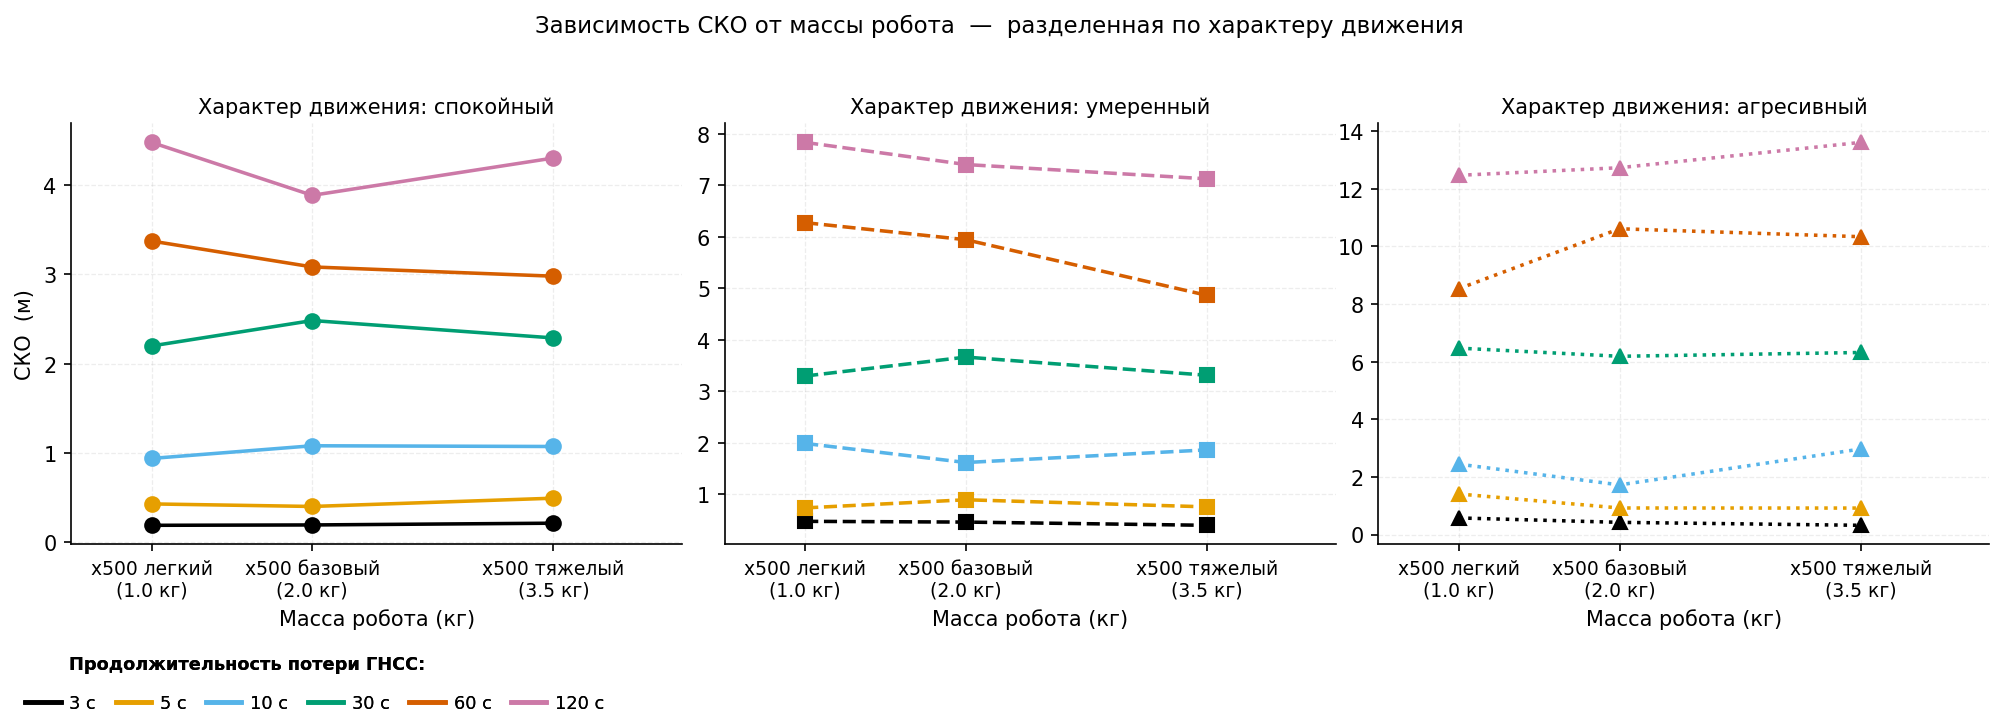
\includegraphics[width=\textwidth]{images/multy_2/plots/rmse_ate_rmse_by_profile.png}
	\caption{Зависимость СКО от массы робота разделенная по характеру движения}
	\label{fig:multy_rmse_profile}
\end{figure}

\begin{figure}[htbp]
	\centering
	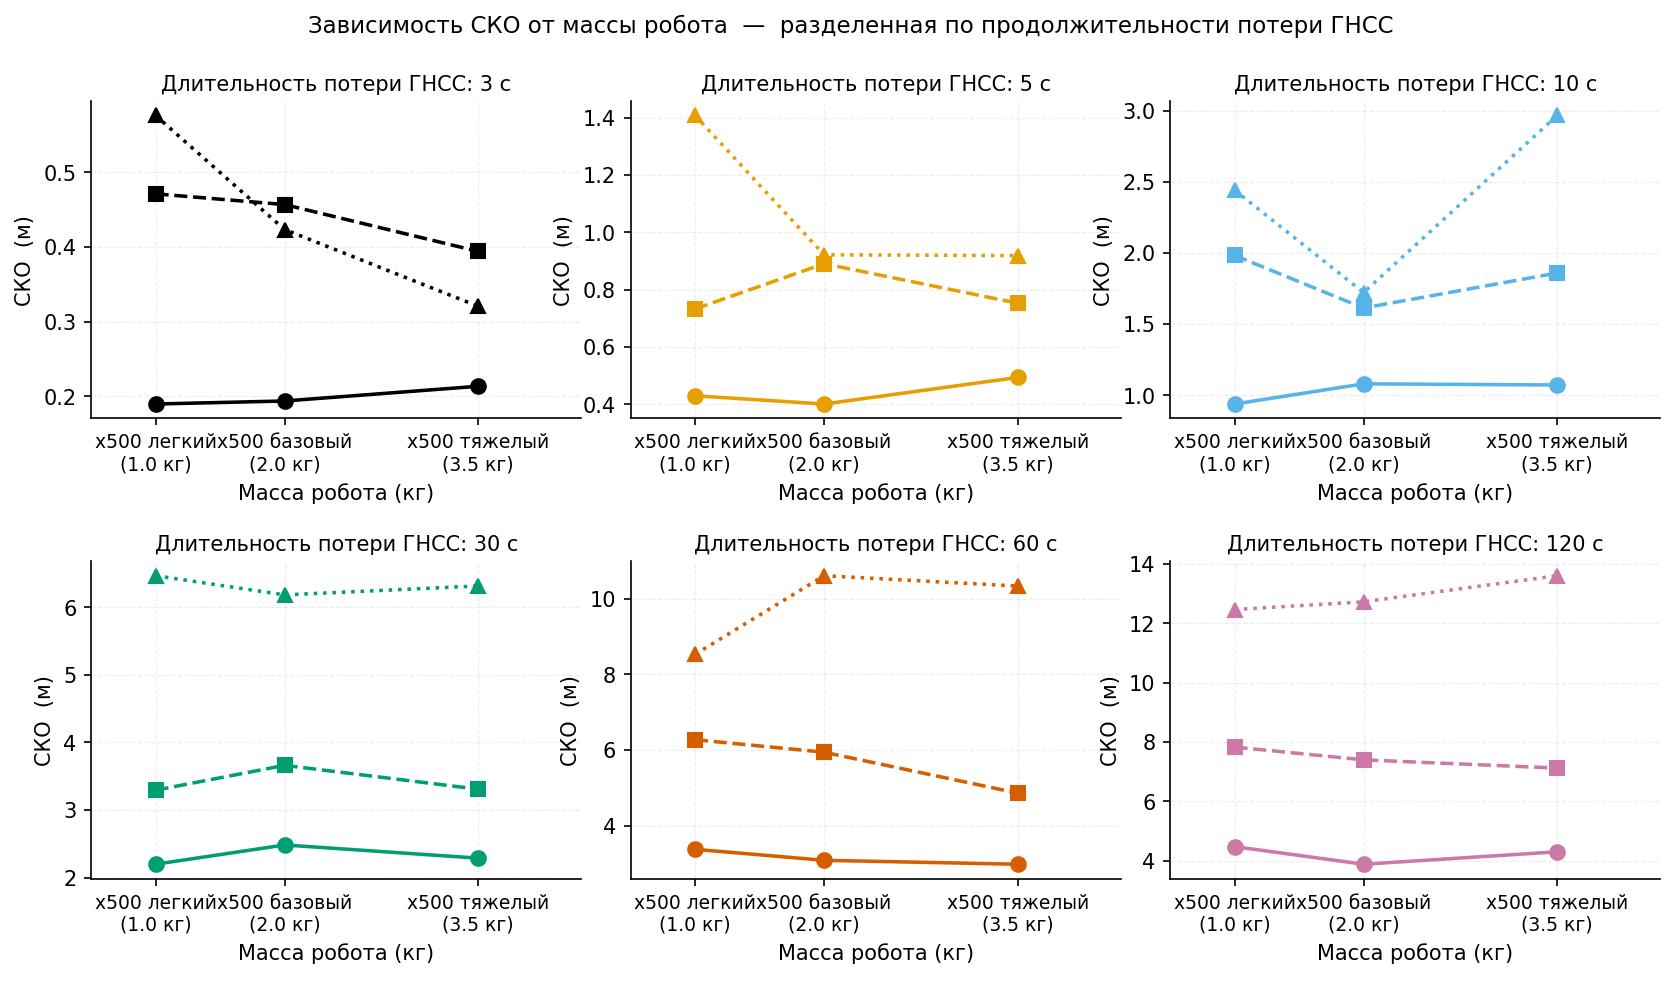
\includegraphics[width=\textwidth]{images/multy_2/plots/rmse_ate_rmse_by_duration.png}
	\caption{Зависимость СКО от массы робота разделенная по длительности потери ГНСС сигнала}
	\label{fig:multy_rmse_duration}
\end{figure}

Из графика \ref{fig:multy_rmse_duration} можно заметить следующие интересные закономерности. 

При длительности потери ГНСС сигнала 3с и агрессивном режиме полета СКО для тяжелого робота 3.5 кг ({0,321} м) меньше чем 
у базовой модели ({0,423} м). Так же СКО при такой же потере сигнала и в том же ре

\subsection{Обсуждение результатов}

Наиболее важный результат эксперимента состоит в том, что обобщение без дообучения ФИ-НС-ПСПС на платформы различной массы оказывается эффективным, особенно при плавных траекториях. При спокойном профиле разброс СКО между платформами при 60 с составляет всего 0,394 м. Это напрямую подтверждает гипотезу, что физическое ограничение на основе оборотов роторов обеспечивает платформенно-инвариантный структурный приоритет.

Тяжёлая платформа в ряде случаев даже превосходит базовую по точности при длительных перерывах. Этому способствуют два фактора. Во-первых, большая инерция сглаживает траектории: даже при агрессивных разворотах изменения скорости происходят более плавно, что облегчает задачу предсказания. Во-вторых, более высокие обороты роторов на висении (около 850 рад/с против 757 рад/с) обеспечивают более сильный и информативный сигнал для вычисления физического остатка.

В то же время агрессивность профиля полёта оказывает существенно большее влияние на точность, чем различия между платформами. Отношение СКО при агрессивном профиле к СКО при спокойном при 60 с находится в диапазоне 2,5--3,5, тогда как вариация между платформами при фиксированном профиле не превышает 20 %. Это означает, что при практическом развёртывании важнее грамотно спроектировать траекторию миссии, чем подбирать конкретную платформу.

Попытки дообучения модели на новых платформах не дали положительного эффекта. Причина — несоответствие статистик нормализации входных признаков. Датасеты лёгкой и тяжёлой платформ имеют иные средние значения и дисперсии оборотов роторов по сравнению с базовым датасетом. При использовании «чужой» нормализации физическая составляющая функции потерь вычисляет некорректные остатки, и градиенты направляют обучение в неверную сторону. 

Этот результат имеет важное практическое значение: корректная нормализация входных данных является обязательным условием успешного переноса обучения в задачах нейросетевой одометрии. Простым и эффективным решением является короткий калибровочный полёт в режиме висения (2--3 минуты) с последующим пересчётом среднего значения и стандартного отклонения сигналов оборотов роторов для целевой платформы.

\subsection{Выводы по разделу}

Проведённый эксперимент по обобщению без дообучения ФИ-НС-ПСПС на три платформы с диапазоном масс 3,5 раза и три профиля полёта (всего 54 условия) позволил сформулировать следующие выводы:

\begin{enumerate}
	\item Обобщение без дообучения является практически применимым. При 10-секундном перерыве ГНСС СКО не превышает 3 м на всех платформах и профилях, что приемлемо для многих прикладных задач.
	
	\item При спокойных траекториях обобщение почти идеально: разброс СКО между платформами при 60 с составляет менее 0,4 м ($<$13 % относительно среднего) несмотря на 3,5-кратный диапазон масс. Это подтверждает платформенную инвариантность физического ограничения на основе оборотов роторов.
	
	\item Тяжёлая платформа в ряде сценариев показывает лучшие результаты при длительных перерывах благодаря сглаживающему эффекту инерции и более сильным сигналам оборотов роторов.
	
	\item Агрессивность миссии оказывает большее влияние на точность, чем различия платформ. При проектировании систем навигации приоритет следует отдавать выбору профиля полёта.
	
	\item Успешный перенос обучения требует предварительной калибровки нормализации входных признаков под целевую платформу. Эта процедура должна входить в стандартный пайплайн развёртывания.
\end{enumerate}	Это взаимодействие между массой платформы и агрессивностью миссии представляет важный нюанс для практиков при проектировании стратегий сбора данных для дообучения.
	
\paragraph{Ограничения.}
Следует отметить несколько ограничений.
	
Во-первых, эксперименты сравнения дообучения модели проведены в симуляции Gazebo. В рамках настоящей работы валидация на реальном оборудовании порведена исключительно на датасете AIIO \cite{AIIO2026}.
	
Во-вторых, масштабирование длины плеча для лёгкой платформы ($l=\SI{0.138}{m}$ против $\SI{0.174}{m}$ у базовой) вносит незначительные изменения в динамическую модель робота.
	
В-третьих, значения СКО при $\tau\geq\SI{60}{s}$ превышают радиус операционной зоны полёта (\SI{70}{m}), поэтому эти метрики отражают асимптотический дрейф, а не практическую ошибку навигации; результаты для коротких потерь сигнала ($\tau\leq\SI{10}{s}$) являются более релевантными с практической точки зрения.
	
	% -----------------------------------------------------------------------------
\section{Заключение}
\label{sec:mp_conclusion}
	
В данной главе представлена систематическая многоплатформенная оценка предложенной архитектуры MambaRPMPINN на трёх конфигурациях квадрокоптера, охватывающих диапазон масс $3{,}5\times$ и три уровня агрессивности полётных миссий.
	
Основные результаты:
	
\begin{enumerate}
	\item \textbf{Дообучение под конкретную платформу эффективно и требует небольшого объёма данных.}
	Пяти эпох на примерно 175\,000 последовательностей на платформу достаточно, чтобы достичь СКО в пределах \SI{22}{m} при потере сигнала ГНСС длительностью \SI{10}{s} для всех трёх платформ по сравнению с диапазоном \SIrange{14}{20}{m} для платформы предобучения.
	\item \textbf{Объединённая стратегия полезна для лёгких платформ, но не для базовой и тяжёлой.}
	Включение кросс-платформенных данных действует как доменная рандомизация для нештатной динамики (лёгкий дрон), но ухудшает точность на платформе предобучения (тяжёлая и базовая конфигурации).
	\item \textbf{Платформенный разрыв масштабирует СКО при умеренных длительностях потери сигнала.}
	Как лёгкая ($\Delta=0{,}5\times$), так и тяжёлая ($\Delta=1{,}75\times$) платформы показывают примерно на 37~\% более высокую среднюю СКО, чем базовая при $\tau=\SI{30}{s}$, подтверждая, что адаптация к массе предобучения является доминирующим фактором.
	\item \textbf{Агрессивность полёта взаимодействует с инерцией платформы.}
	Влияние профиля уменьшается с ростом массы платформы — от отношения $1{,}87\times$ (спокойный/агрессивный) для лёгкой платформы до всего $1{,}05\times$ для тяжёлой. Это указывает на то, что платформы с высокой инерцией inherently более устойчивы к вариациям профиля миссии в наборе данных для дообучения.
\end{enumerate}
	
Эти результаты подтверждают подход физически информированного трансферного обучения для одометрии квадрокоптеров и дают количественные рекомендации для практиков при выборе данных для дообучения при развёртывании предложенной системы на новой платформе.
	
\section{Обобщение без дообучения ФИ-НС-ПСПС на платформы различной массы и динамики}
\label{sec:mp_crossplatform}

В предыдущих разделах главы было показано, что предлагаемая физически информированная нейросетевая система позиционирования (ФИ-НС-ПСПС) на базе архитектуры Mamba с регуляризатором на основе оборотов роторов обеспечивает точную инерциальную одометрию при перерывах в приёме сигналов ГНСС на квадрокоптере Holybro X500~V2. Однако для практического внедрения принципиально важно понять, насколько эта система способна обобщаться на другие платформы без дополнительного обучения. 

Большинство современных подходов к восстановлению траектории по данным инерциальных датчиков фактически запоминают статистические особенности шумов и динамики конкретного аппарата. Эти особенности напрямую зависят от массы, моментов инерции и аэродинамических характеристик, поэтому модель, обученная на одном квадрокоптере, обычно не может быть напрямую перенесена на другой без дообучения. 

В отличие от чисто data-driven решений, в ФИ-НС-ПСПС явно присутствует физическое ограничение, соответствующее второму закону Ньютона:
\begin{equation}
	m\,\mathbf{a} =
	\sum_{i=1}^{4} k_T\,\omega_i^2\,\hat{\mathbf{z}}_{\mathrm{body}}
	- b_{\mathrm{drag}}\,m\,\mathbf{v}
	+ m\,\mathbf{g},
	\label{eq:newton_full}
\end{equation}
где $m$ — масса платформы, $k_T$ — коэффициент тяги мотора, $\omega_i$ — угловые скорости роторов, $b_{\mathrm{drag}}$ — коэффициент аэродинамического сопротивления, $\mathbf{v}$ — скорость центра масс в связанной системе координат, $\mathbf{g}$ — ускорение свободного падения. 

Эта зависимость имеет одинаковую структуру для любого жёсткого квадрокоптера; изменяются лишь числовые значения массы и коэффициента тяги. Гипотеза, проверяемая в данном разделе, заключается в том, что нейросетевая часть системы в первую очередь выучивает отображение, определяемое именно этой инвариантной физической структурой, а влияние массы на результат поглощается через наблюдаемые сигналы оборотов роторов.

Для проверки гипотезы был проведён эксперимент по обобщению без дообучения. Предобученная ФИ-НС-ПСПС оценивалась на трёх платформах, охватывающих диапазон масс 3,5 раза, и на трёх профилях полёта с различной агрессивностью — без какого-либо дообучения под целевую платформу. 

\subsection{Описание экспериментальных платформ}

В качестве базовой использовалась модель Holybro X500~V2 — та же платформа, на которой проводились все предыдущие эксперименты. На её основе были созданы две дополнительные виртуальные платформы путём изменения только инерционных параметров при сохранении неизменными характеристик моторов, пропеллеров и состава датчиков. Такой подход позволяет изолировать влияние массы и инерции на точность одометрии.

\textbf{Лёгкая платформа.} Масса рамы 1,0 кг, длина плеча 0,138 м. Соответствует минимальной комплектации X500~V2 без полезной нагрузки и близка по характеристикам к компактным исследовательским квадрокоптерам класса 250--330 мм.

\textbf{Тяжёлая платформа.} Масса рамы 3,5 кг, длина плеча 0,210 м. Имитирует аппарат с полезной нагрузкой около 1,5 кг (например, лидар или тепловизионная камера) — типичная конфигурация для задач промышленного мониторинга. Коэффициент тяги мотора увеличен до $1{,}188 \times 10^{-5}$ для сохранения достаточного запаса тяги на висении.

Полный перечень физических и имитационных параметров трёх платформ приведён в таблице~\ref{tab:platforms_full}.

\begin{table}[htbp]
	\centering
	\footnotesize
	\caption{Физические и имитационные параметры экспериментальных платформ. Параметры, отличающиеся от базовой, выделены жирным шрифтом. Разрыв платформы $\Delta = m / m_{\mathrm{base}}$ характеризует величину доменного сдвига.}
	\label{tab:platforms_full}
	\setlength{\tabcolsep}{3pt}
	\resizebox{0.97\textwidth}{!}{%
		\begin{tabular}{llccc}
			\toprule
			\textbf{Параметр} & \textbf{Ед. изм.} &
			\textbf{Базовая} & \textbf{Лёгкая} & \textbf{Тяжёлая} \\
			\midrule
			\multicolumn{5}{l}{\textit{Физические параметры}} \\
			Масса рамы $m$ & кг & 2{,}0 & \textbf{1{,}0} & \textbf{3{,}5} \\
			Момент инерции $I_{xx}=I_{yy}$ & кг·м$^2$ & 0{,}02167 & \textbf{0{,}00683} & \textbf{0{,}05507} \\
			Момент инерции $I_{zz}$ & кг·м$^2$ & 0{,}04000 & \textbf{0{,}01260} & \textbf{0{,}10165} \\
			Длина плеча $l$ & м & 0{,}174 & \textbf{0{,}138} & \textbf{0{,}210} \\
			\midrule
			\multicolumn{5}{l}{\textit{Параметры силовой установки}} \\
			Коэффициент тяги $k_T$ & Н/(рад/с)$^2$ & $8{,}549\times10^{-6}$ & $8{,}549\times10^{-6}$ & $\mathbf{1{,}188\times10^{-5}}$ \\
			Коэффициент сопротивления вращению $k_D$ & Н·м/(рад/с)$^2$ & $1{,}368\times10^{-7}$ & $1{,}368\times10^{-7}$ & $\mathbf{1{,}901\times10^{-7}}$ \\
			Постоянная времени набора оборотов $\tau_{\uparrow}$ & с & 0{,}0125 & \textbf{0{,}0088} & \textbf{0{,}0165} \\
			Постоянная времени сброса оборотов $\tau_{\downarrow}$ & с & 0{,}0250 & \textbf{0{,}0177} & \textbf{0{,}0331} \\
			\midrule
			\multicolumn{5}{l}{\textit{Параметры системы управления}} \\
			Тяга на висении \texttt{MPC\_THR\_HOVER} & -- & 0{,}60 & \textbf{0{,}54} & \textbf{0{,}85} \\
			Идентификатор airframe \texttt{SYS\_AUTOSTART} & -- & 4001 & \textbf{4022} & \textbf{4023} \\
			\midrule
			\multicolumn{5}{l}{\textit{Производные характеристики}} \\
			Разрыв платформы $\Delta$ & -- & $1{,}0\times$ & $\mathbf{0{,}5\times}$ & $\mathbf{1{,}75\times}$ \\
			Тяга одного мотора на висении $mg/4$ & Н & 4{,}905 & \textbf{2{,}452} & \textbf{8{,}584} \\
			Обороты роторов на висении $\omega_h$ & рад/с & 757 & \textbf{535} & \textbf{850} \\
			Отношение тяги к весу $T/W$ & -- & 1{,}74 & \textbf{3{,}48} & \textbf{1{,}37} \\
			\bottomrule
		\end{tabular}%
	}
\end{table}

Таблица~\ref{tab:platform_realworld} показывает соответствие имитационных моделей реальным аналогам.

\begin{table}[htbp]
	\centering
	\footnotesize
	\caption{Соответствие имитационных моделей реальным платформам.}
	\label{tab:platform_realworld}
	\setlength{\tabcolsep}{3pt}
	\resizebox{0.95\textwidth}{!}{%
		\begin{tabular}{llp{5.5cm}}
			\toprule
			\textbf{Имитационная модель} & \textbf{Реальная платформа} & \textbf{Основные сходства} \\
			\midrule
			Базовая & Holybro X500~V2 + Pixhawk 6C + батарея 4S 5000 мА·ч & Полное совпадение \\
			Лёгкая & X500~V2 в минимальной комплектации; класс DJI F330 & Масса около 1 кг, рама 250--330 мм \\
			Тяжёлая & X500~V2 с полезной нагрузкой 1,5 кг (лидар) & Масса 3--4 кг, тяжеловесная конфигурация \\
			\bottomrule
		\end{tabular}%
	}
\end{table}


\subsection{Профили полётных заданий}

Для эксперимента были сформированы три профиля полёта, различающиеся скоростью, высотой и минимальным углом разворота (таблица~\ref{tab:mission_profiles}). Все платформы использовали одни и те же траектории, поэтому наблюдаемые различия в точности обусловлены исключительно динамическими свойствами аппаратов.

\begin{table}[htbp]
	\centering
	\footnotesize
	\caption{Параметры профилей полётных заданий. Минимальный угол разворота обеспечивает резкие изменения курса и увеличивает разницу оборотов между парами роторов.}
	\label{tab:mission_profiles}
	\setlength{\tabcolsep}{3pt}
	\resizebox{0.97\textwidth}{!}{%
		\begin{tabular}{lccccc}
			\toprule
			\textbf{Профиль} & \textbf{Max. скорость, м/с} & \textbf{Высота, м} &
			\textbf{Мин. угол разворота} & \textbf{Количество точек} & \textbf{Радиус зоны, м} \\
			\midrule
			Спокойный   & 8  & 8--20  & --          & 50 & 40 \\
			Умеренный   & 12 & 5--35  & $\geq 45^\circ$  & 50 & 60 \\
			Агрессивный & 15 & 5--45  & $\geq 90^\circ$  & 50 & 70 \\
			\bottomrule
		\end{tabular}%
	}
\end{table}
\subsection{Методика проведения эксперимента}

Для каждой из девяти комбинаций (три платформы × три профиля) выполнялся полёт в среде PX4 SITL с использованием Gazebo. Из полученных логов извлекались показания гироскопа, акселерометра, магнитометра, кватернион ориентации, команды на моторы (в пересчёте на угловые скорости роторов) и эталонные положение и скорость из EKF2. Данные ресемплировались до частоты 100 Гц. Участки ниже высоты 1 м и буферы взлёта/посадки исключались. Перерывы в приёме сигналов ГНСС длительностью 10 с (по 20 на каждый лог) имитировались маскированием соответствующих измерений. 

Размеры сформированных датасетов после предобработки приведены в таблице~\ref{tab:dataset_sizes}.

\begin{table}[htbp]
	\centering
	\caption{Объёмы датасетов после предобработки (количество отсчётов при частоте 100 Гц примерно соответствует секундам полёта).}
	\label{tab:dataset_sizes}
	\begin{tabular}{lrrrr}
		\toprule
		\textbf{Платформа} & \textbf{Спокойный} & \textbf{Умеренный} &
		\textbf{Агрессивный} & \textbf{Итого} \\
		\midrule
		Базовая        & 43\,536 & 52\,693 & 79\,738 & 175\,967 \\
		Лёгкая & 43\,819 & 53\,138 & 80\,479 & 177\,436 \\
		Тяжёлая & 43\,222 & 51\,960 & 79\,039 & 174\,221 \\
		\midrule
		\textbf{Всего}       & 130\,577 & 157\,791 & 239\,256 & 527\,624 \\
		\bottomrule
	\end{tabular}
\end{table}

Перед оценкой на каждой новой платформе в модель подставлялись соответствующие физические параметры (масса, коэффициент тяги, длина плеча) без изменения весов нейросети. Это единственная адаптация, выполнявшаяся в эксперименте.

Оценка проводилась по единой методике. Для каждого лога выбиралось 10 случайных начальных позиций. Предсказанные скорости интегрировались методом Рунге—Кутты четвёртого порядка с двунаправленным сглаживанием. Использовались две метрики без применения выравнивания по методу Умеямы:
\begin{align}
	\text{СКО} &= \sqrt{\frac{1}{3T}\sum_{t=1}^{T}\|\hat{\mathbf{p}}_t - \mathbf{p}_t\|^2}, \\
	\text{АОТ} &= \frac{1}{T}\sum_{t=1}^{T}\|\hat{\mathbf{p}}_t - \mathbf{p}_t\|_2.
\end{align}
Длительности перерывов в приёме сигналов ГНСС: 3, 5, 10, 30, 60 и 120 с.

\subsection{Результаты эксперимента}

Полные значения СКО и АОТ для всех комбинаций платформ и профилей полёта приведены в таблицах~\ref{tab:rmse_full} и~\ref{tab:ate_full}. Эти данные составляют основной количественный результат раздела.

\begin{table}[htbp]
	\centering
	\footnotesize
	\caption{Среднеквадратичная ошибка положения (СКО, м) для всех комбинаций платформа--профиль и длительностей перерывов ГНСС. Обобщение без дообучения. Лучшее значение в каждом столбце подчеркнуто.}
	\label{tab:rmse_full}
	\setlength{\tabcolsep}{3pt}
	\resizebox{0.98\textwidth}{!}{%
		\begin{tabular}{llrrrrrr}
			\toprule
			\textbf{Платформа} & \textbf{Профиль} &
			\textbf{3 с} & \textbf{5 с} & \textbf{10 с} &
			\textbf{30 с} & \textbf{60 с} & \textbf{120 с} \\
			\midrule
			\multirow{3}{*}{Базовая}
			& спокойный   & \underline{0{,}194} & 0{,}401 & 1{,}081 & 2{,}483 &  3{,}083 &  3{,}885 \\
			& умеренный   & 0{,}457 & 0{,}890 & 1{,}613 & 3{,}661 &  5{,}940 &  7{,}400 \\
			& агрессивный & 0{,}423 & 0{,}921 & 1{,}722 & 6{,}183 & 10{,}606 & 12{,}723 \\
			\midrule
			\multirow{3}{*}{Лёгкая}
			& спокойный   & 0{,}190 & 0{,}429 & \underline{0{,}939} & \underline{2{,}198} &  3{,}373 &  4{,}478 \\
			& умеренный   & 0{,}471 & 0{,}732 & 1{,}983 & 3{,}293 &  6{,}271 &  7{,}830 \\
			& агрессивный & 0{,}576 & 1{,}407 & 2{,}442 & 6{,}466 &  8{,}527 & 12{,}460 \\
			\midrule
			\multirow{3}{*}{Тяжёлая}
			& спокойный   & 0{,}214 & 0{,}494 & 1{,}072 & 2{,}288 &  \underline{2{,}979} &  \underline{4{,}303} \\
			& умеренный   & \underline{0{,}394} & \underline{0{,}752} & 1{,}860 & \underline{3{,}308} &  \underline{4{,}859} &  \underline{7{,}122} \\
			& агрессивный & \underline{0{,}321} & \underline{0{,}918} & 2{,}967 & 6{,}315 & 10{,}331 & 13{,}602 \\
			\bottomrule
		\end{tabular}%
	}
\end{table}

Анализ скорости роста ошибки (отношение СКО при 60 с к СКО при 10 с) показал, что тяжёлая платформа демонстрирует наименьшие темпы накопления ошибки при спокойном и умеренном профилях.

Анализ зависимости точности от разрыва платформы (отношения массы к базовой) выявил важную закономерность: при длительности перерыва 30--60 с кривая зависимости СКО от разрыва платформы становится практически плоской. Это означает, что обобщение без дообучения работает почти одинаково хорошо на всех трёх платформах, несмотря на 3,5-кратный диапазон масс.

Особенно показательны результаты при спокойном профиле полёта (таблица~\ref{tab:calm_crossplatform}). Разброс значений СКО между платформами при 60 с не превышает 0,394 м, что составляет менее 13 процентов относительно среднего значения. Это исключительно малое различие при изменении массы в 3,5 раза.

\begin{table}[htbp]
	\centering
	\caption{Среднеквадратичная ошибка положения при спокойном профиле полёта. Разброс между платформами (максимум минус минимум) остаётся ниже 0,5 м даже при 60-секундном перерыве ГНСС.}
	\label{tab:calm_crossplatform}
	\begin{tabular}{rrrrrr}
		\toprule
		\textbf{Длительность} & \textbf{Базовая} & \textbf{Лёгкая} &
		\textbf{Тяжёлая} & \textbf{Разброс} \\
		\midrule
		3 с   & 0{,}194 & 0{,}190 & 0{,}214 & 0{,}024 \\
		5 с   & 0{,}401 & 0{,}429 & 0{,}494 & 0{,}093 \\
		10 с  & 1{,}081 & 0{,}939 & 1{,}072 & 0{,}142 \\
		30 с  & 2{,}483 & 2{,}198 & 2{,}288 & 0{,}285 \\
		60 с  & 3{,}083 & 3{,}373 & 2{,}979 & 0{,}394 \\
		120 с & 3{,}885 & 4{,}478 & 4{,}303 & 0{,}593 \\
		\bottomrule
	\end{tabular}
\end{table}

На рисунках \ref{fig:multy_rmse_profile} и \ref{fig:multy_rmse_duration} приведены графики зависимость СКО от массы робота. 

\begin{figure}[htbp]
	\centering
	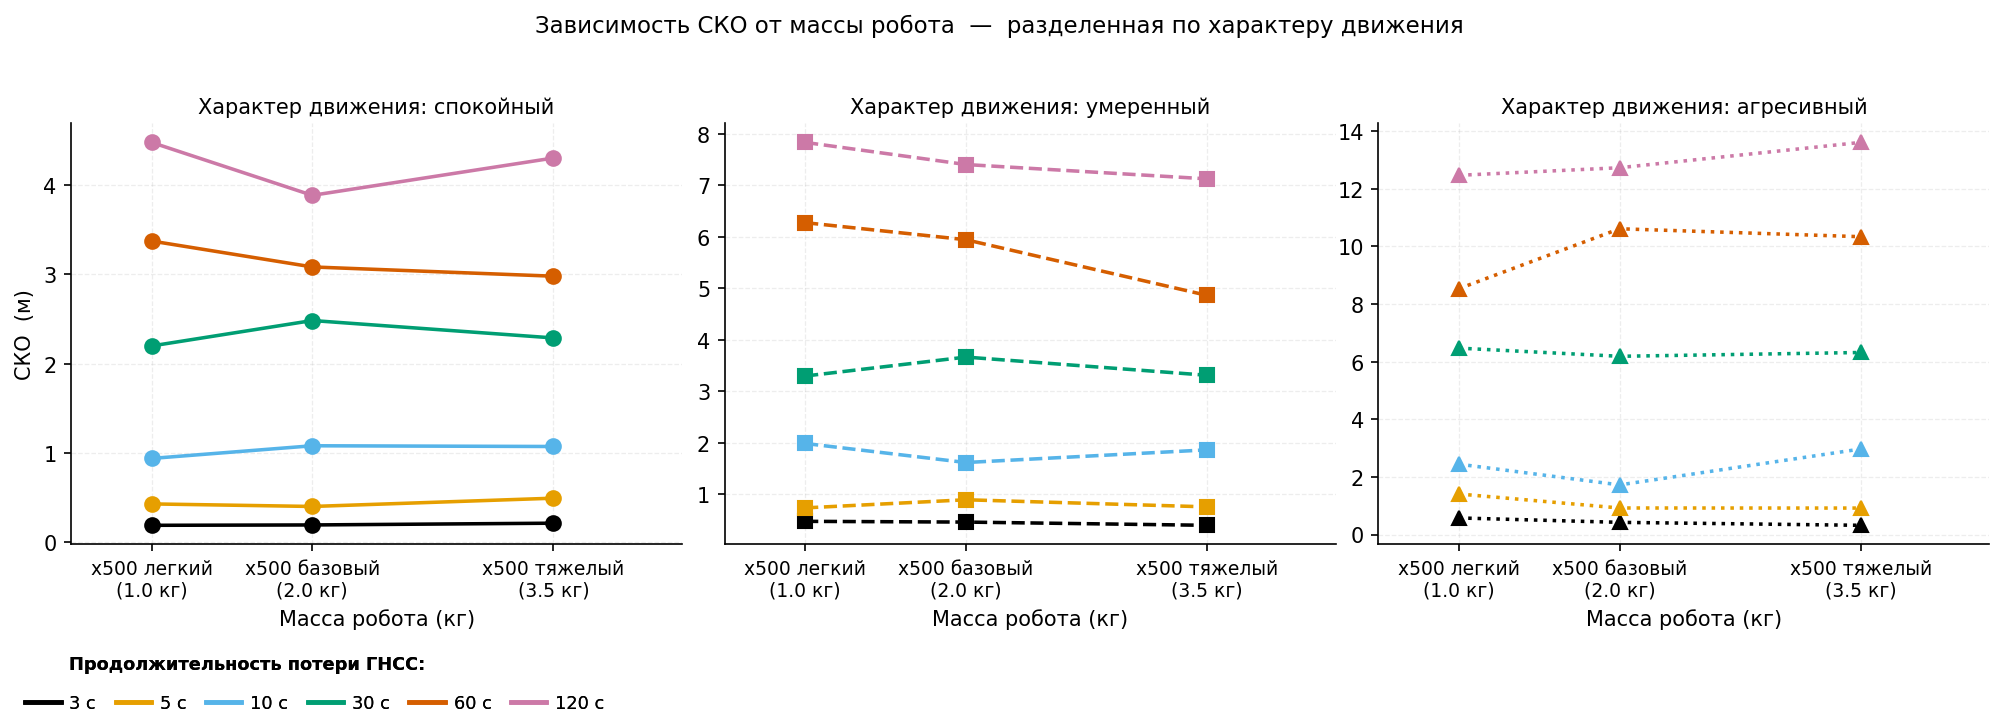
\includegraphics[width=\textwidth]{images/multy_2/plots/rmse_ate_rmse_by_profile.png}
	\caption{Зависимость СКО от массы робота разделенная по характеру движения}
	\label{fig:multy_rmse_profile}
\end{figure}

\begin{figure}[htbp]
	\centering
	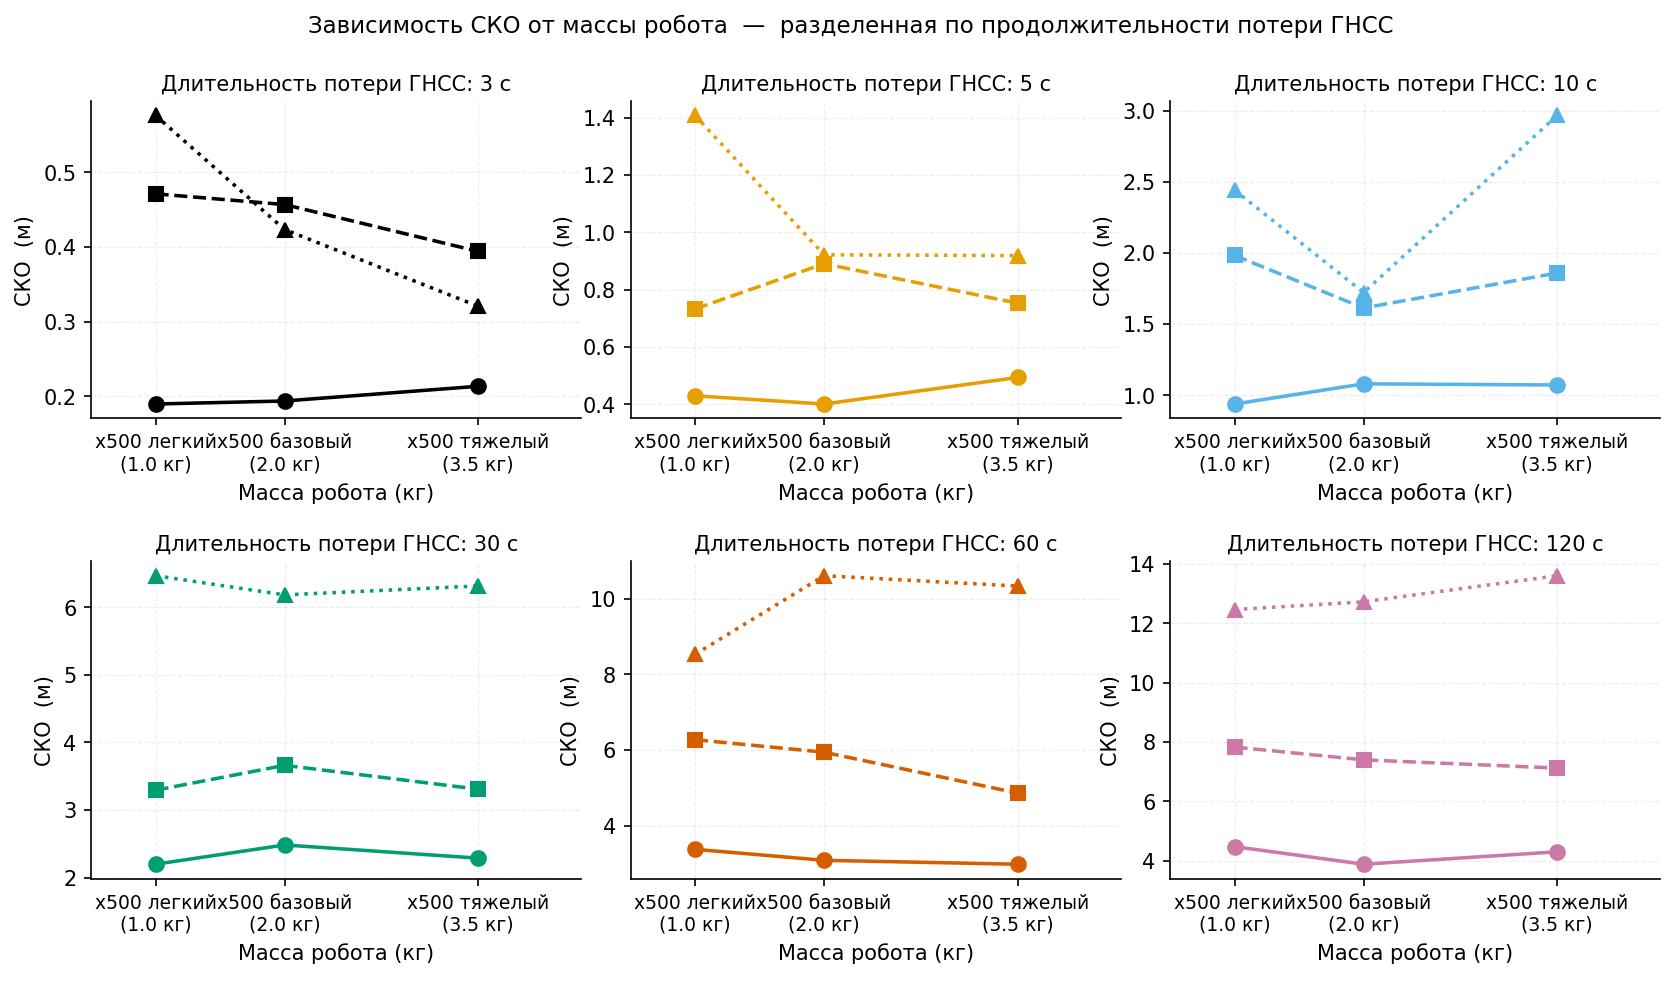
\includegraphics[width=\textwidth]{images/multy_2/plots/rmse_ate_rmse_by_duration.png}
	\caption{Зависимость СКО от массы робота разделенная по длительности потери ГНСС сигнала}
	\label{fig:multy_rmse_duration}
\end{figure}

Из графика \ref{fig:multy_rmse_duration} можно заметить следующие интересные закономерности. 

При длительности потери ГНСС сигнала 3с и агрессивном режиме полета СКО для тяжелого робота 3.5 кг ({0,321} м) меньше чем 
у базовой модели ({0,423} м). Так же СКО при такой же потере сигнала и в том же ре

\subsection{Обсуждение результатов}

Наиболее важный результат эксперимента состоит в том, что обобщение без дообучения ФИ-НС-ПСПС на платформы различной массы оказывается эффективным, особенно при плавных траекториях. При спокойном профиле разброс СКО между платформами при 60 с составляет всего 0,394 м. Это напрямую подтверждает гипотезу, что физическое ограничение на основе оборотов роторов обеспечивает платформенно-инвариантный структурный приоритет.

Тяжёлая платформа в ряде случаев даже превосходит базовую по точности при длительных перерывах. Этому способствуют два фактора. Во-первых, большая инерция сглаживает траектории: даже при агрессивных разворотах изменения скорости происходят более плавно, что облегчает задачу предсказания. Во-вторых, более высокие обороты роторов на висении (около 850 рад/с против 757 рад/с) обеспечивают более сильный и информативный сигнал для вычисления физического остатка.

В то же время агрессивность профиля полёта оказывает существенно большее влияние на точность, чем различия между платформами. Отношение СКО при агрессивном профиле к СКО при спокойном при 60 с находится в диапазоне 2,5--3,5, тогда как вариация между платформами при фиксированном профиле не превышает 20 %. Это означает, что при практическом развёртывании важнее грамотно спроектировать траекторию миссии, чем подбирать конкретную платформу.

Попытки дообучения модели на новых платформах не дали положительного эффекта. Причина — несоответствие статистик нормализации входных признаков. Датасеты лёгкой и тяжёлой платформ имеют иные средние значения и дисперсии оборотов роторов по сравнению с базовым датасетом. При использовании «чужой» нормализации физическая составляющая функции потерь вычисляет некорректные остатки, и градиенты направляют обучение в неверную сторону. 

Этот результат имеет важное практическое значение: корректная нормализация входных данных является обязательным условием успешного переноса обучения в задачах нейросетевой одометрии. Простым и эффективным решением является короткий калибровочный полёт в режиме висения (2--3 минуты) с последующим пересчётом среднего значения и стандартного отклонения сигналов оборотов роторов для целевой платформы.

\subsection{Выводы по разделу}

Проведённый эксперимент по обобщению без дообучения ФИ-НС-ПСПС на три платформы с диапазоном масс 3,5 раза и три профиля полёта (всего 54 условия) позволил сформулировать следующие выводы:

\begin{enumerate}
	\item Обобщение без дообучения является практически применимым. При 10-секундном перерыве ГНСС СКО не превышает 3 м на всех платформах и профилях, что приемлемо для многих прикладных задач.
	
	\item При спокойных траекториях обобщение почти идеально: разброс СКО между платформами при 60 с составляет менее 0,4 м ($<$13 % относительно среднего) несмотря на 3,5-кратный диапазон масс. Это подтверждает платформенную инвариантность физического ограничения на основе оборотов роторов.
	
	\item Тяжёлая платформа в ряде сценариев показывает лучшие результаты при длительных перерывах благодаря сглаживающему эффекту инерции и более сильным сигналам оборотов роторов.
	
	\item Агрессивность миссии оказывает большее влияние на точность, чем различия платформ. При проектировании систем навигации приоритет следует отдавать выбору профиля полёта.
	
	\item Успешный перенос обучения требует предварительной калибровки нормализации входных признаков под целевую платформу. Эта процедура должна входить в стандартный пайплайн развёртывания.
\end{enumerate}	


\subsection{Обсуждение результатов кросс-платформенного обобщения без дообучения}
\label{subsec:mp_discussion}

На рисунке \ref{fig:rmse_mass_profile} приведены зависимости СКО от длительности потери сигнала ГНСС. 

\begin{figure}[htbp]
	\centering
	\includegraphics[width=\textwidth]{images/multy_2/plots/rmse_vs_duration.png}
	\caption{Зависимость  СКО от длительности потери сигнала ГНСС}
	\label{fig:rmse_mass_profile}
\end{figure}

Эксперимент по оценке способности ФИ-НС-ПСПС к обобщению без дообучения проводился на трёх виртуальных платформах, различающихся массой в 3,5 раза, при трёх профилях полёта различной агрессивности. Модель, предобученная исключительно на базовой платформе массой 2,0~кг, оценивалась на лёгкой (1,0~кг) и тяжёлой (3,5~кг) платформах без какой-либо адаптации весов. Ниже обсуждаются наиболее значимые результаты, полученные при анализе зависимостей среднеквадратической ошибки от длительности перерыва ГНСС (рисунок~\ref{fig:rmse_mass_profile}).

\begin{itemize}
	\item \textbf{Тяжёлая платформа демонстрирует преимущество при длительных перерывах ГНСС.}  
	При outage 60~с тяжёлая платформа (3,5~кг) показывает меньшую ошибку, чем базовая, на 18~\% в умеренном профиле и до 20~\% лучше лёгкой платформы в агрессивном режиме. Эффект проявляется только при длительности перерыва свыше 30~с и усиливается с ростом outage. Данный результат представляется неочевидным, поскольку модель обучалась на платформе вдвое меньшей массы. Наиболее вероятными причинами являются два фактора, непосредственно вытекающие из динамической модели квадрокоптера (глава~2). Во-первых, большая инерция тяжёлой платформы приводит к более плавным изменениям линейной скорости даже при резких командах на разворот; такие траектории легче предсказывать методом последовательного интегрирования. Во-вторых, более высокие обороты роторов на висении (примерно 850~рад/с против 757~рад/с у базовой платформы) обеспечивают более сильный и информативный сигнал для вычисления физического остатка в функционале потерь~\eqref{eq:loss_df}. Таким образом, физический регуляризатор на основе телеметрии оборотов несущих винтов оказывается более эффективным именно на платформах с большей массой.
	
	\item \textbf{Базовая платформа (платформа предобучения) показывает наихудший темп накопления ошибки при агрессивном профиле.}  
	Отношение СКО при 60~с к СКО при 10~с для агрессивного режима составило 6,16 для базовой платформы против 3,48–3,49 для лёгкой и тяжёлой. Этот результат является парадоксальным: модель, обученная именно на базовой платформе, демонстрирует наиболее быстрое ухудшение точности при длительных агрессивных манёврах. Лёгкая и тяжёлая платформы при этом ведут себя практически идентично. Данное наблюдение может свидетельствовать о том, что в процессе обучения модель в определённой степени «подстроилась» под статистические особенности именно базовой платформы, тогда как более инерционные или более «проворные» платформы порождают траектории, лучше соответствующие обобщающим свойствам архитектуры ФИ-НС-ПСПС.
	
	\item \textbf{Разброс точности между платформами немонотонно зависит от длительности перерыва.}  
	При агрессивном профиле на длительности 30~с значения СКО для всех трёх платформ практически совпадают (в диапазоне 6,2–6,5~м), тогда как при 10~с и 60~с разброс существенно больше. Природа этого «схлопывания» на отметке 30~с пока не имеет однозначного объяснения. Можно предположить связь с характерным временным масштабом двунаправленного сглаживания методом Рунге—Кутты четвёртого порядка с линейным blending, однако данный вопрос требует отдельного исследования.
	
	\item \textbf{Отношение АОТ к СКО остаётся практически постоянным во всех условиях.}  
	Значение АОТ/СКО лежит в узком диапазоне 1,50–1,57 для всех 54 комбинаций платформы, профиля полёта и длительности перерыва ГНСС. Это указывает на то, что геометрическая структура ошибки предсказания траектории самоподобна и не зависит от динамических свойств платформы. Ошибка, по-видимому, определяется преимущественно систематическим смещением в оценке скорости, а не случайным накоплением дрейфа. Данное наблюдение подтверждает, что физический регуляризатор действительно ограничивает пространство допустимых решений модели, делая характер ошибок более предсказуемым и интерпретируемым.
	
	\item \textbf{Агрессивность профиля полёта оказывает существенно большее влияние на точность, чем различия между платформами.}  
	Разница между спокойным и агрессивным профилями при outage 60~с достигает фактора 3,4× на базовой платформе, тогда как вариация между платформами при фиксированном профиле не превышает 20~\% (для спокойного режима). Это означает, что при практическом развёртывании системы приоритет следует отдавать выбору и проектированию траектории миссии, а не подбору конкретной платформы.
\end{itemize}

Полученные результаты позволяют сформулировать следующие практические выводы. Во-первых, обобщение без дообучения для ФИ-НС-ПСПС является работоспособным в диапазоне изменения массы платформы до 3,5 раз при условии, что длительность перерыва ГНСС не превышает 30~с. Во-вторых, успешность переноса существенно зависит от динамического режима полёта: при спокойных траекториях обобщение почти идеально, тогда как агрессивные манёвры требуют либо дообучения, либо более консервативного планирования миссии. В-третьих, корректная нормализация входных признаков (в первую очередь оборотов роторов) под целевую платформу является обязательным условием успешного применения метода. Простейшим практическим решением является короткий калибровочный полёт в режиме висения продолжительностью 2–3~минуты с последующим пересчётом среднего значения и стандартного отклонения сигналов оборотов.

Таким образом, физический регуляризатор на основе телеметрии оборотов несущих винтов обеспечивает не только повышение точности на одной платформе, но и определённую платформенную инвариантность модели, что является важным преимуществом для практического внедрения в условиях ограниченного объёма данных.


\section{Выводы по главе}
\label{sec:ch4_conclusions}

В четвёртой главе проведено экспериментальное исследование физически информированной нейросетевой системы восстановления траектории квадрокоптера при кратковременных потерях сигнала ГНСС. Основные результаты состоят в следующем.

1. Разработан и реализован протокол дообучения на ограниченном объёме данных режима компенсации порывов ветра. Показано, что при дообучении на 25~\% данных (соответствует примерно 2~минутам полёта) предлагаемая ФИ-НС-ПСПС достигает СКО 9,4~м при outage 240~с, что в 1,8 раза лучше, чем у базовой нейронной сети, обученной на полном датасете. Физический регуляризатор на основе закона тяги несущих винтов обеспечивает повышенный контраст обучающего сигнала именно в условиях высокой дисперсии оборотов роторов, что позволяет эффективно адаптировать модель к новому динамическому режиму при минимальном объёме калибровочных данных.

2. Проведено систематическое сравнение четырёх архитектур (ФИ-НС-ПСПС, обобщённая НС-ПСПС, базовая НС-ПСПС и Transformer) на задаче восстановления траектории. ФИ-НС-ПСПС устойчиво превосходит остальные модели при всех долях дообучающих данных и всех длительностях перерыва ГНСС, при этом сохраняя линейную вычислительную сложность, характерную для архитектур семейства Mamba.

3. Выполнено исследование кросс-платформенного обобщения без дообучения на трёх платформах с диапазоном масс 3,5 раза и трёх профилях полёта различной агрессивности. Установлено, что обобщение является практически применимым: при outage 10~с СКО не превышает 3~м на всех платформах и профилях. При спокойных траекториях разброс СКО между платформами при 60~с составляет менее 0,4~м, что подтверждает платформенную инвариантность физического ограничения. Выявлены неочевидные эффекты: тяжёлая платформа в ряде сценариев превосходит базовую при длительных перерывах благодаря сглаживающему действию инерции и более сильному сигналу оборотов роторов; базовая платформа (платформа предобучения) показывает наихудший темп накопления ошибки при агрессивном профиле; отношение АОТ к СКО остаётся практически постоянным (1,50–1,57) во всех условиях, что указывает на структурный характер ошибки.

4. Установлено, что агрессивность профиля полёта оказывает существенно большее влияние на точность восстановления траектории, чем различия между платформами. При проектировании систем навигации приоритет следует отдавать выбору и планированию траектории миссии.

5. Выявлена критическая роль корректной нормализации входных признаков при переносе обучения. Некорректная нормализация предотвращает сходимость дообучения даже при наличии предобученной модели. Разработана практическая рекомендация: перед применением на новой платформе выполнять короткий калибровочный полёт в режиме висения с последующим пересчётом статистик нормализации.

Полученные результаты подтверждают эффективность предложенного подхода, сочетающего архитектуру с селективными пространствами состояний и физический регуляризатор на основе телеметрии оборотов несущих винтов, как для задач дообучения на малых данных, так и для кросс-платформенного переноса без дообучения.